%!TEX root = ../../thesis.tex
\define{\chapterpath}{\allchapterspath/bci}
\define{\imgpath}{\chapterpath/img}

\chapter{Application to Brain Computer Interaction}
\label{chapter:bci}
\minitoc

We have presented an algorithm that exploits task constraints to solve simultaneously a task under human feedback and learn the associated meanings of the feedback signals. We have detailed an uncertainty measure than allow our agent to solve this problem more efficiently and shown that our algorithm can transition from task to task in a smooth way. This has important practical application since the user can start controlling a device from scratch, without the need of an expert to define the meaning of signals or carrying out a calibration phase. 

In this section, we explore the use of our algorithm to the brain computer interaction following the same reaching task scenario as presented in chapter~\ref{chapter:planning:method}. After discussing the related work, we will first test our algorithm with a database of EEG signals and compare its performance with a calibration procedure method that first collect known signal-label pair and train a unique classifier. We will present one experiment in more details and show that our algorithm conserve good properties on EEG signals and has important advantage over calibration based method. 

However we will point out a main difference between calibration procedure and our self-calibration method in that the EEG signals properties can be affected by the action of the agent. As our planning method can not guarantee the same agent behavior than during the calibration procedure, the quality of the signal received by the users can be impacted. To address this problem we will introduce a prior information of the Error-related potential EEG signals used, namely that the signal corresponding to an ``incorrect'' meaning are more ``powerful'' than the one associated to meaning ``correct''. We will exploit this properties, in addition to our interpretation hypothesis method, and show that we can achieve better performances. We finally present results where different users teach an agent to reach a particular state by assessing the agent action in their mind, and without calibrating the system before hand.

Those results with real EEG signals allow us to believe such algorithm could have practical application into the real word. By removing the user of an expert to collect and calibrate the system, we may democratize the use of brain computer interface and allow their users to go out of the labs. However there is number of limitation that would need to be addressed, such as the synchronous interactions assumption, the discrete state, discrete action. Most of the current limitation of this work will be addressed in the next section.

The application of this work to BCI is a collaboration with I{\~n}aki Iturrate and Luis Montesano.

%%%%%%%%%%%%%%%%%%%%%%%%%%%%%%%%%%%%%%%%%%%%%%
%%%%%%%%%%%%%%%%%%%%%%%%%%%%%%%%%%%%%%%%%%%%%%
%%%%%%%%%%%%%%%%%%%%%%%%%%%%%%%%%%%%%%%%%%%%%%
%%%%%%%%%%%%%%%%%%%%%%%%%%%%%%%%%%%%%%%%%%%%%%
%%%%%%%%%%%%%%%%%%%%%%%%%%%%%%%%%%%%%%%%%%%%%%
\section{Using pre-recorded EEG signals}
\label{chapter:bci:EEGsignals}

We want to apply our algorithm to BCI scenario, before trying out on real subject we tested the feasibility of the proposed self-calibration approach using real ErrP datasets. The objective of this analysis is to study the scalability of our method to EEG data, which may have different properties than our artificial dataset. We will see that our algorithm conserve good properties using EEG signals.

\subsection{Dataset and scenario}

\paragraph{EEG datasets}  The EEG data were recorded in a previous study \cite{iturrate2013task} where participants monitored on a screen the execution of a task where a virtual device had to reach a given goal. The motion of the device could be correct (towards the goal) or erroneous (away from the goal). The subjects were asked to mentally assess the device movements as erroneous or non-erroneous. The EEG signals were recorded with a gTec system with 32 electrodes distributed according to an extended 10/20 international system with the ground on FPz and the reference on the left earlobe. The ErrP features were extracted from two fronto-central channels (FCz and Cz) within a time window of $[200,700]$ ms (being 0 ms the action onset of the agent) and downsampled to $32$ Hz. This leaded to a vector of $34$ features.

Note that the scenario used to collect the EEG data is the same as the one we run in our simulated experiment and is the same as the one we will run in our online experiment with real subjects.

\paragraph{Comparison with calibration methods} In order to show the benefit of learning without explicit calibration, we compare our method with the standard supervised BCI calibration procedure. In this calibration procedure, which can last for up to 40 minutes, the experimenter needs to record enough data from the user from several offline runs, where the user is not controlling the agent but just passively assessing its actions. Following the literature on ErrPs \cite{chavarriaga2010learning,iturrate2013task} our training data will consist of 80 percent of positive examples (associated to a correct feedback) and 20 percent of negative examples (associated to an incorrect feedback). Our proposed algorithm is compared with different (but standard) sizes of calibration datasets: 200, 300 and 400 examples.

\subsection{One example detailed}

Figure~\ref{fig:sequence} shows one particular run of 500 steps comparing our self-calibration method with a calibration procedure of 400 steps. The two independent runs use a real EEG dataset with $80\%$ ten-fold classification accuracy. As our algorithm is operational from the first step, it can estimate the real task when sufficient evidence has been collected. On the other hand, a calibration approach collects signal-label pairs for a fixed number of steps and use the resulting classifier without updating it. This provokes that, during the calibration phase, no tasks can be learned, substantially delaying the user's online operation. 

Of important interest is the ability of the algorithm to evaluate when sufficient evidence has been collected. The dataset considered is relatively good quality, and we do not need 400 steps to identify the first task. When doing a calibration procedure, the experiment can not known in advance the quality of each particular subject. Therefore, he must run a calibration for long enough so as to have enough data point to adapt to all possible data quality. However, for some subject collecting 100 sample is enough.

\begin{figure}[!htbp]
\centering
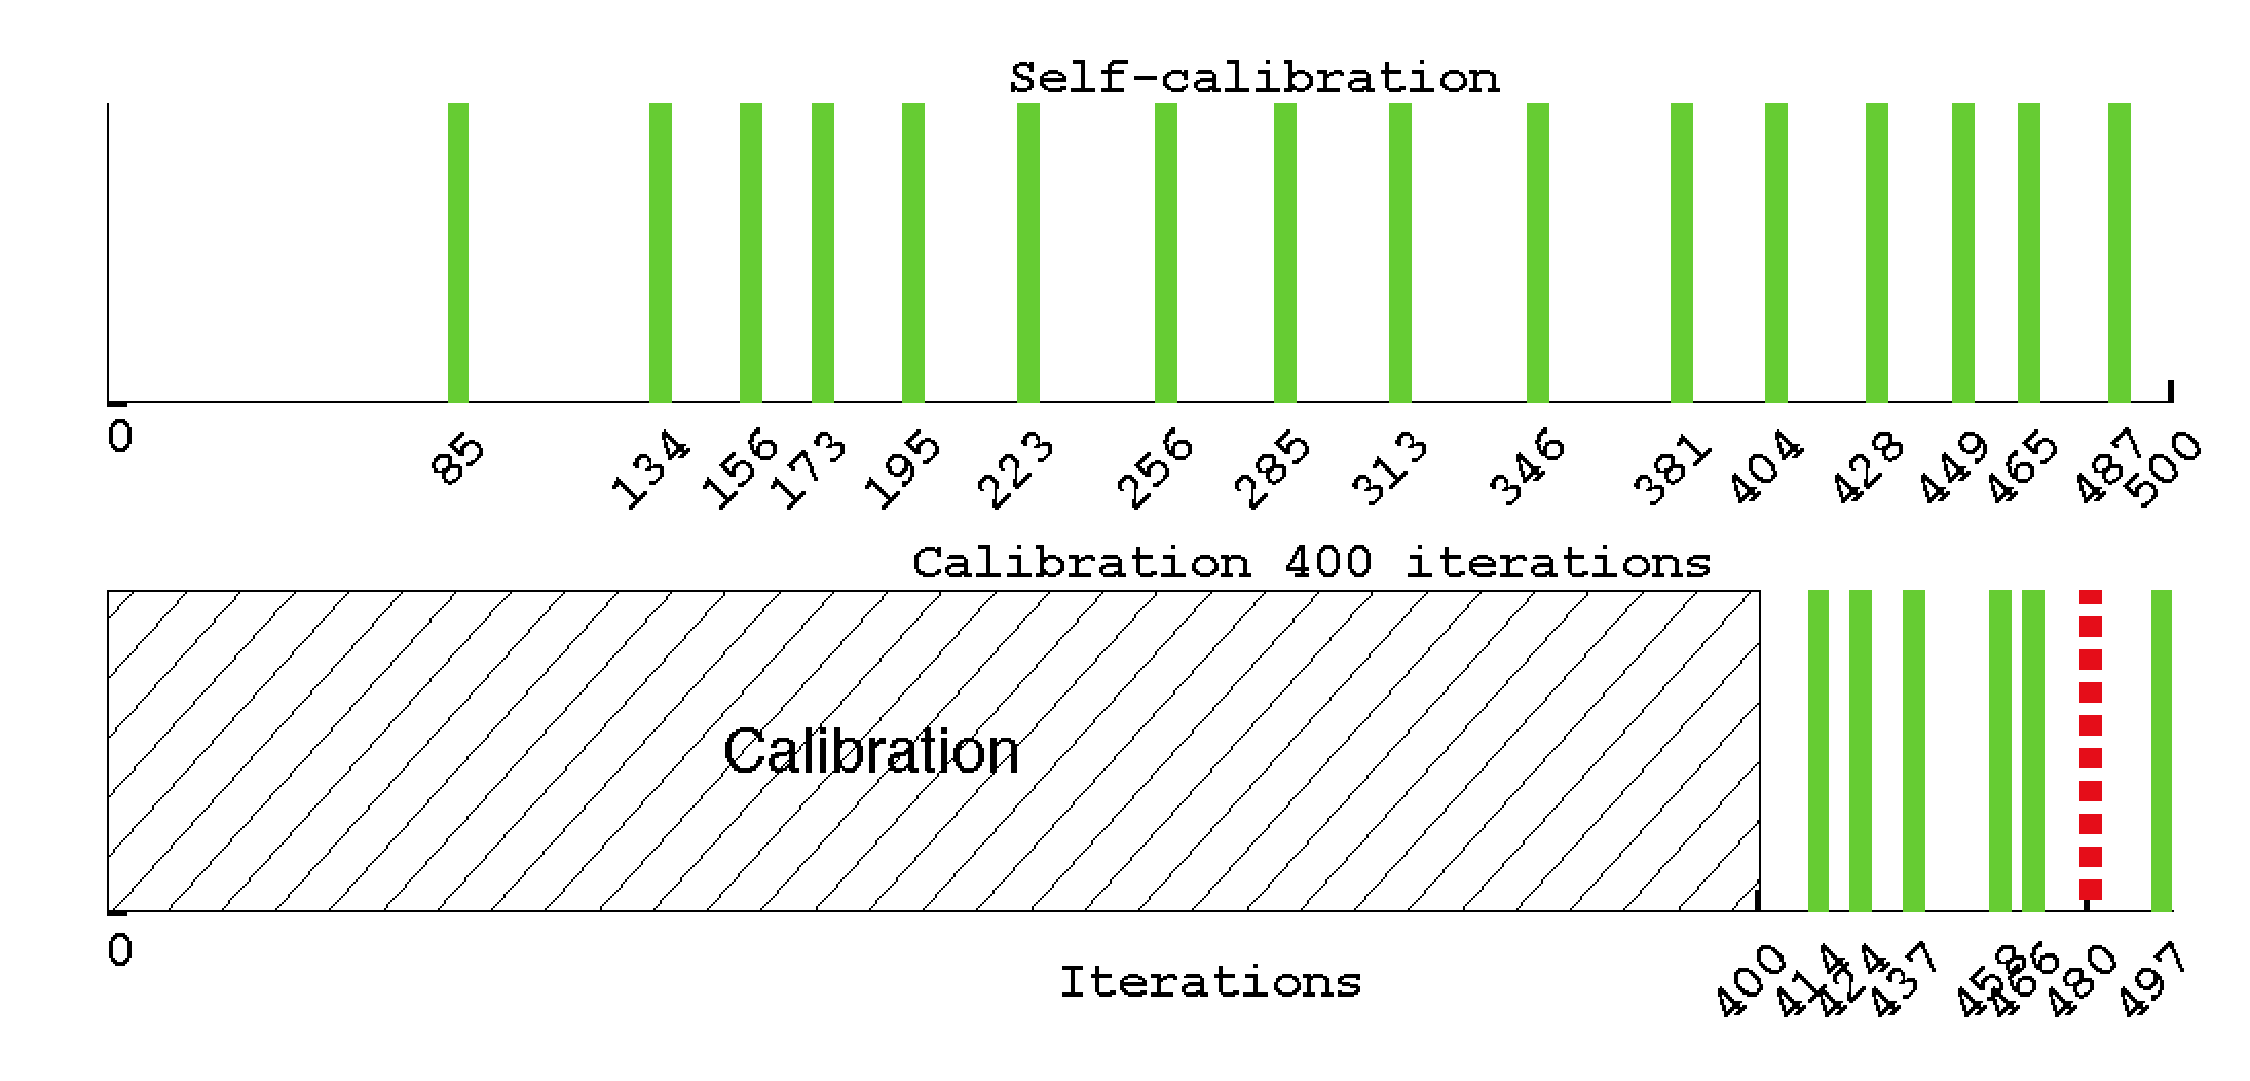
\includegraphics[width=\sequencesize\columnwidth]{\imgpath/plot_the_aaai_sequence.eps}
\caption{Time-line of one run from EEG dataset of $80$ percent ten-fold classification accuracy, self-calibration (top) versus 400 steps calibration (bottom). Green (filled) and red (dashed) bars represents respectively correct and incorrect task achievement. The proposed self-calibration method allow to reach a first task faster than would take a calibration procedure.}
\label{fig:sequence}
\end{figure} 


Figure~\ref{fig:sequence_evolution} shows the evolution of classification rate between our self-calibration method with a calibration procedure of 400 steps. As our method assigns different labels to each new teaching signal, the resulting classifiers have different performances, which help identifying the correct task. Once a task is identified (e.g.\ step 85 and 134), and as explained in chapter~\ref{chapter:lfui:tasttotask} the corresponding labels are taken as ground truth, and all classifiers will have the same accuracies. As the agent starts exploring again to estimate the new tasks, all the classifiers except the true one will start to have worse accuracies again.

\begin{figure}[!htbp]
\centering
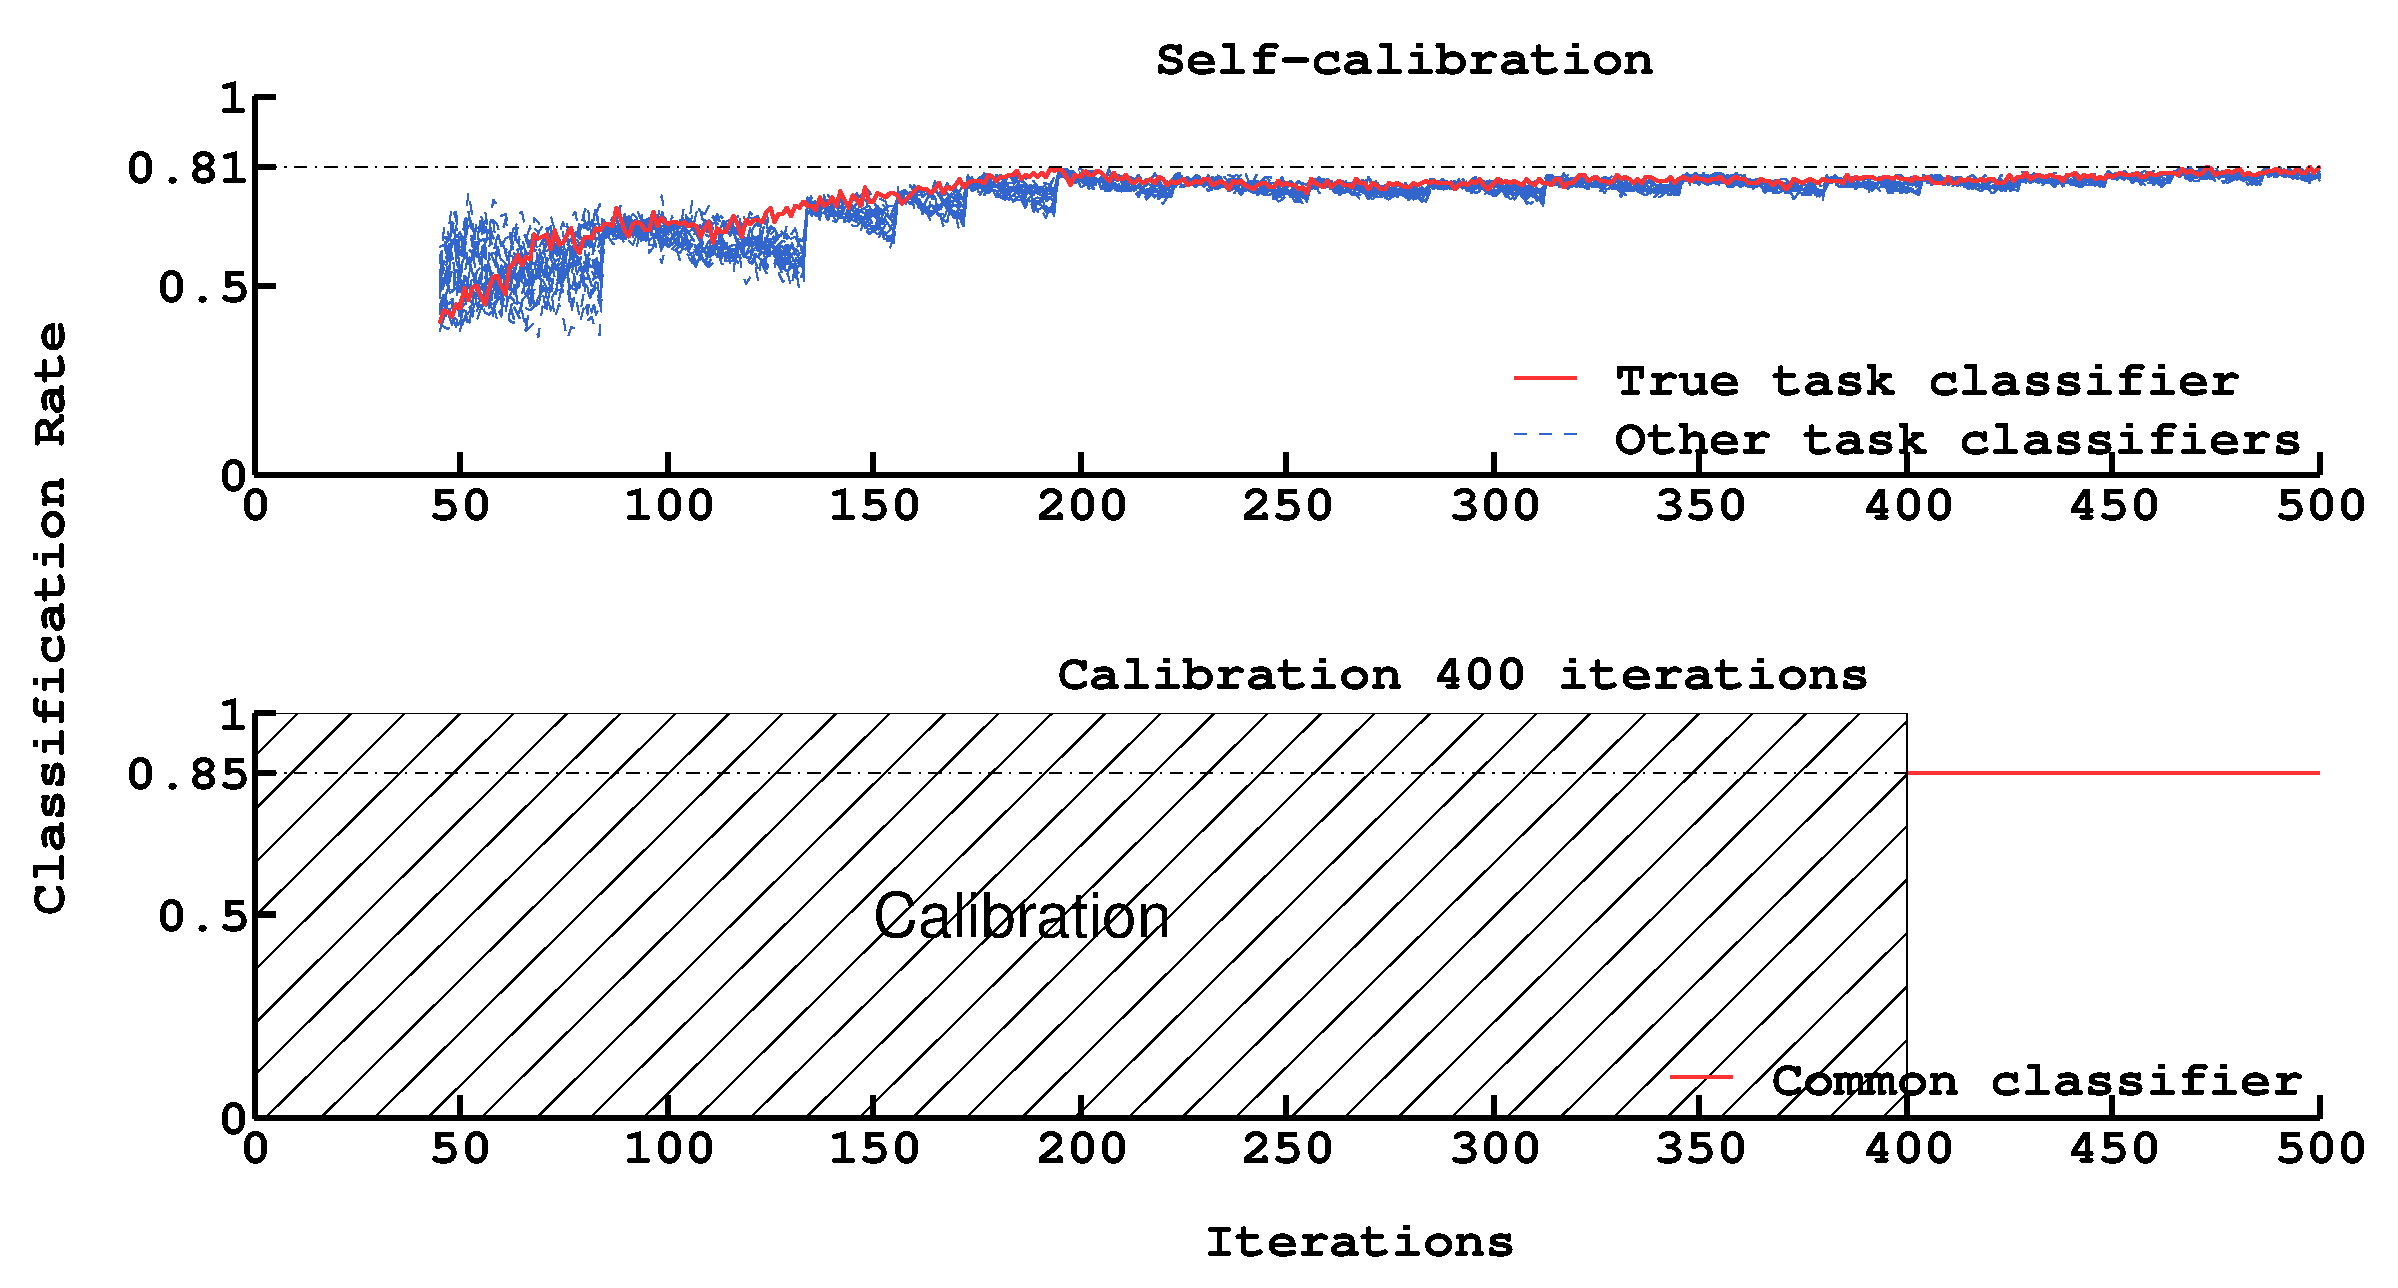
\includegraphics[width=\sequencesize\columnwidth]{\imgpath/plot_evo_classification_rate.eps}
\caption{Evolution of classification rate of one run from EEG data, self-calibration (top) versus 400 steps calibration (bottom). On top, the red line represents the classifier corresponding to the successive tasks taught by the user, the dashed blue lines represent all others tasks. Our method updates classifiers every steps.}
\label{fig:sequence_evolution}
\end{figure} 

We can observe here the continuous transition between what we called phase 1 and phase 2 in chapter~\ref{chapter:lfui:rephrasing}. We remind here that we are using Equation~\ref{eq:matchingfiltercrossvalidation} to compute the likelihood of each task using a 10 fold cross-validation to compute the confusion matrix.

Before the step 200, we observe a strong evolution of every classifiers (see Figure~\ref{fig:sequence_evolution} top), during this phase the algorithm do not have enough data to create a good classifier of the data and rely mainly on the hypothetic labeling process to differentiate between hypothesis. For example at step 130, the classifier corresponding to the true task is of better quality that all the other one, therefore, via the estimation of its confusion matrix, its estimates are more considered than the update from the other hypothesis. 

However after step 200, the difference between classifier qualities is very small as they now share most of their signal-label pairs (due to the propagation of label after each task identified (see chapter~\ref{chapter:lfui:tasttotask}). From that point the algorithm is very similar than using a calibrated classifier common for all hypothesis, we differentiate between hypothesis on a point by point basis. Indeed as all hypothesis make similar predictions, hypothesis whose predicted labels match with the expected labels see their probabilities increased. Respectively, hypothesis whose predicted labels do not match with the expected labels see their probabilities decreased.

Interestingly those two phases are captured by the same equation (see Equation~\ref{eq:matchingcrossvalidation}) which compares predicted and expected labels while taking into account the confidence in the prediction of each classifier through the estimated confusion matrix.

\subsection{Planning}

Figure~\ref{fig:planningEEG} compares the number of steps (with maximum values of 500 steps) needed to identify the first task when learning from scratch with different planning methods. Our proposed planning method leads the system towards regions that maximize disambiguation among hypotheses and outperforms the other action selection methods. Those results are in line with the one using artificial datasets in Figure~\ref{fig:artificialplanning}. Given these results, the remainder of this section will only consider our planning method.


\begin{figure}[!htbp]
    \centering
    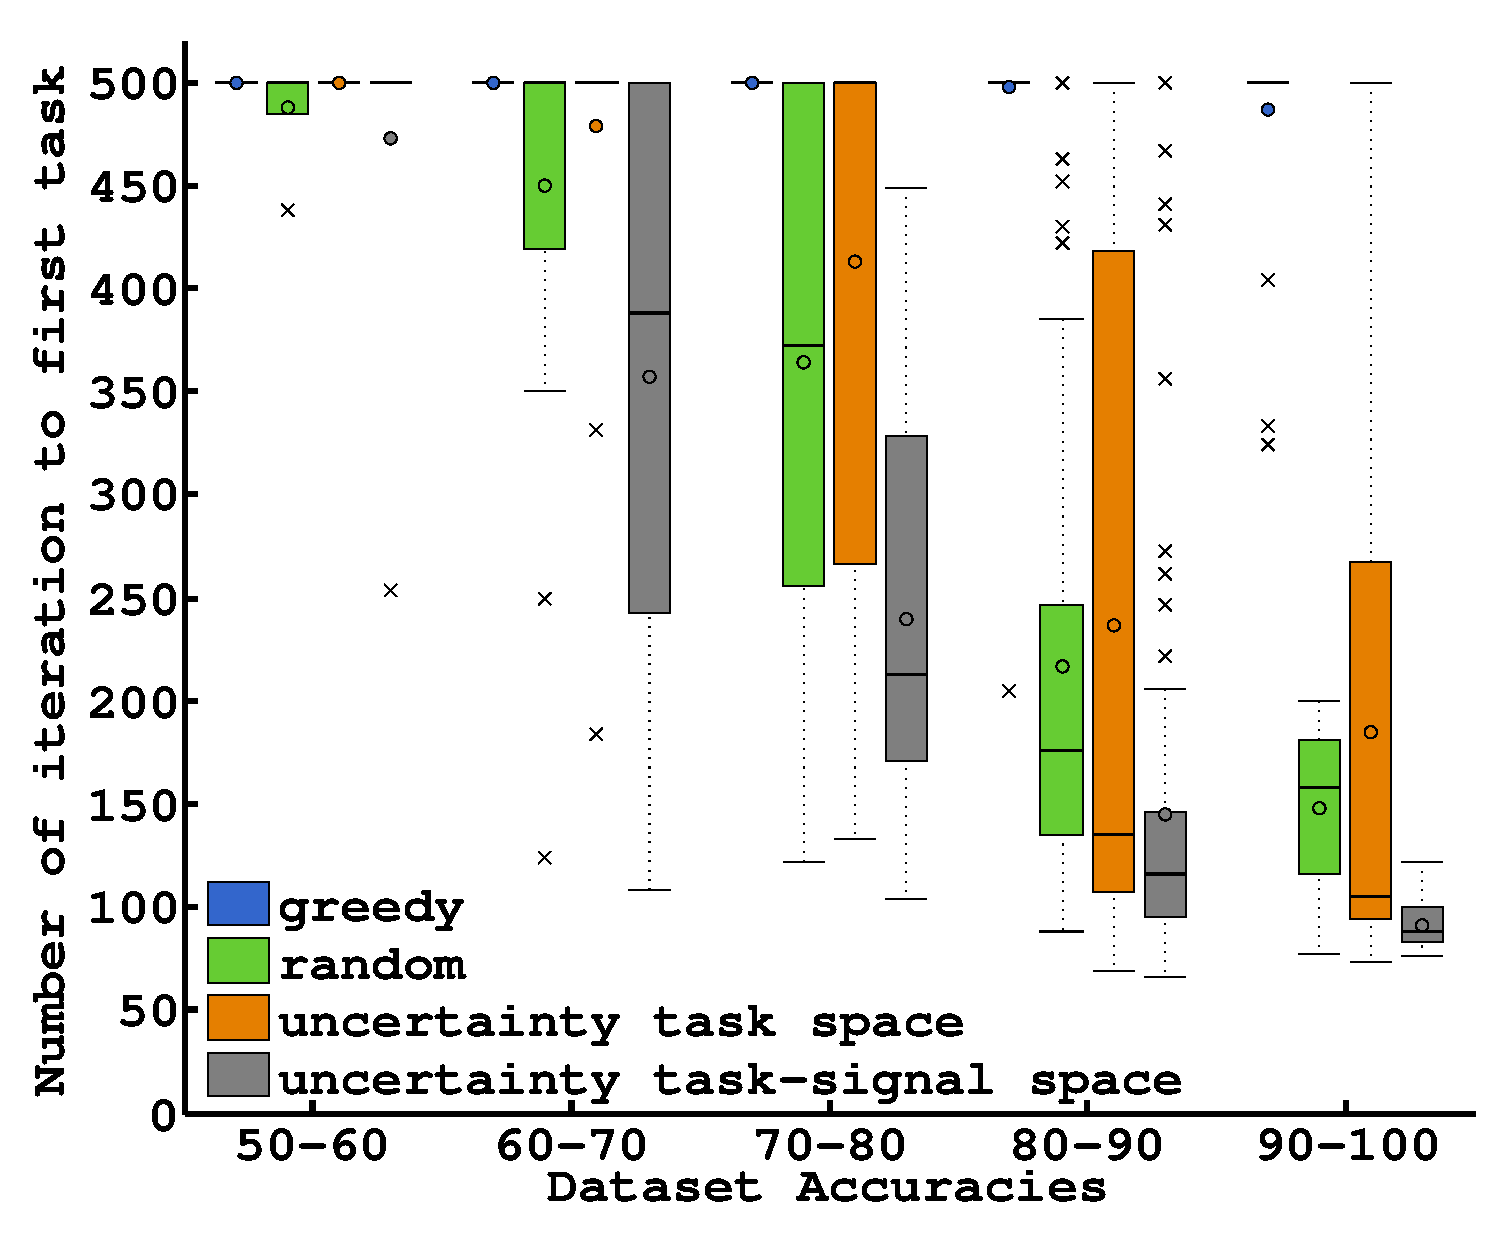
\includegraphics[width=\plotsize\columnwidth]{\imgpath/plot_EEG_planning.eps}
    \caption{Number of steps to complete first task using EEG data of different quality. The EEG data have similar properties than our 30 dimensional simulated data in Figure~\ref{fig:artificialplanning}. Our planning method based on both the task and the signal to meaning mapping uncertainty is more efficient that choosing action randomly, greedily or only based on the uncertainty on the task.}
    \label{fig:planningEEG}
\end{figure}

\subsection{Time to first task}

Figure~\ref{fig:firstEEG} shows the number of iterations to identify the first task and compares the results between our self-calibration method and calibration period of 200, 300, and 400 iterations. The percentage of time the task first task was correct is show on top of the each box plot. For our self-calibration method, the learning time is strongly correlated with the dataset quality. This is an important properties as we are able to adapt online to the quality of the data we receive. For dataset of more than 80 percent classification rate, we can complete the first task is less than 150 steps on average without mistake.

\begin{figure}[!htbp]
\centering
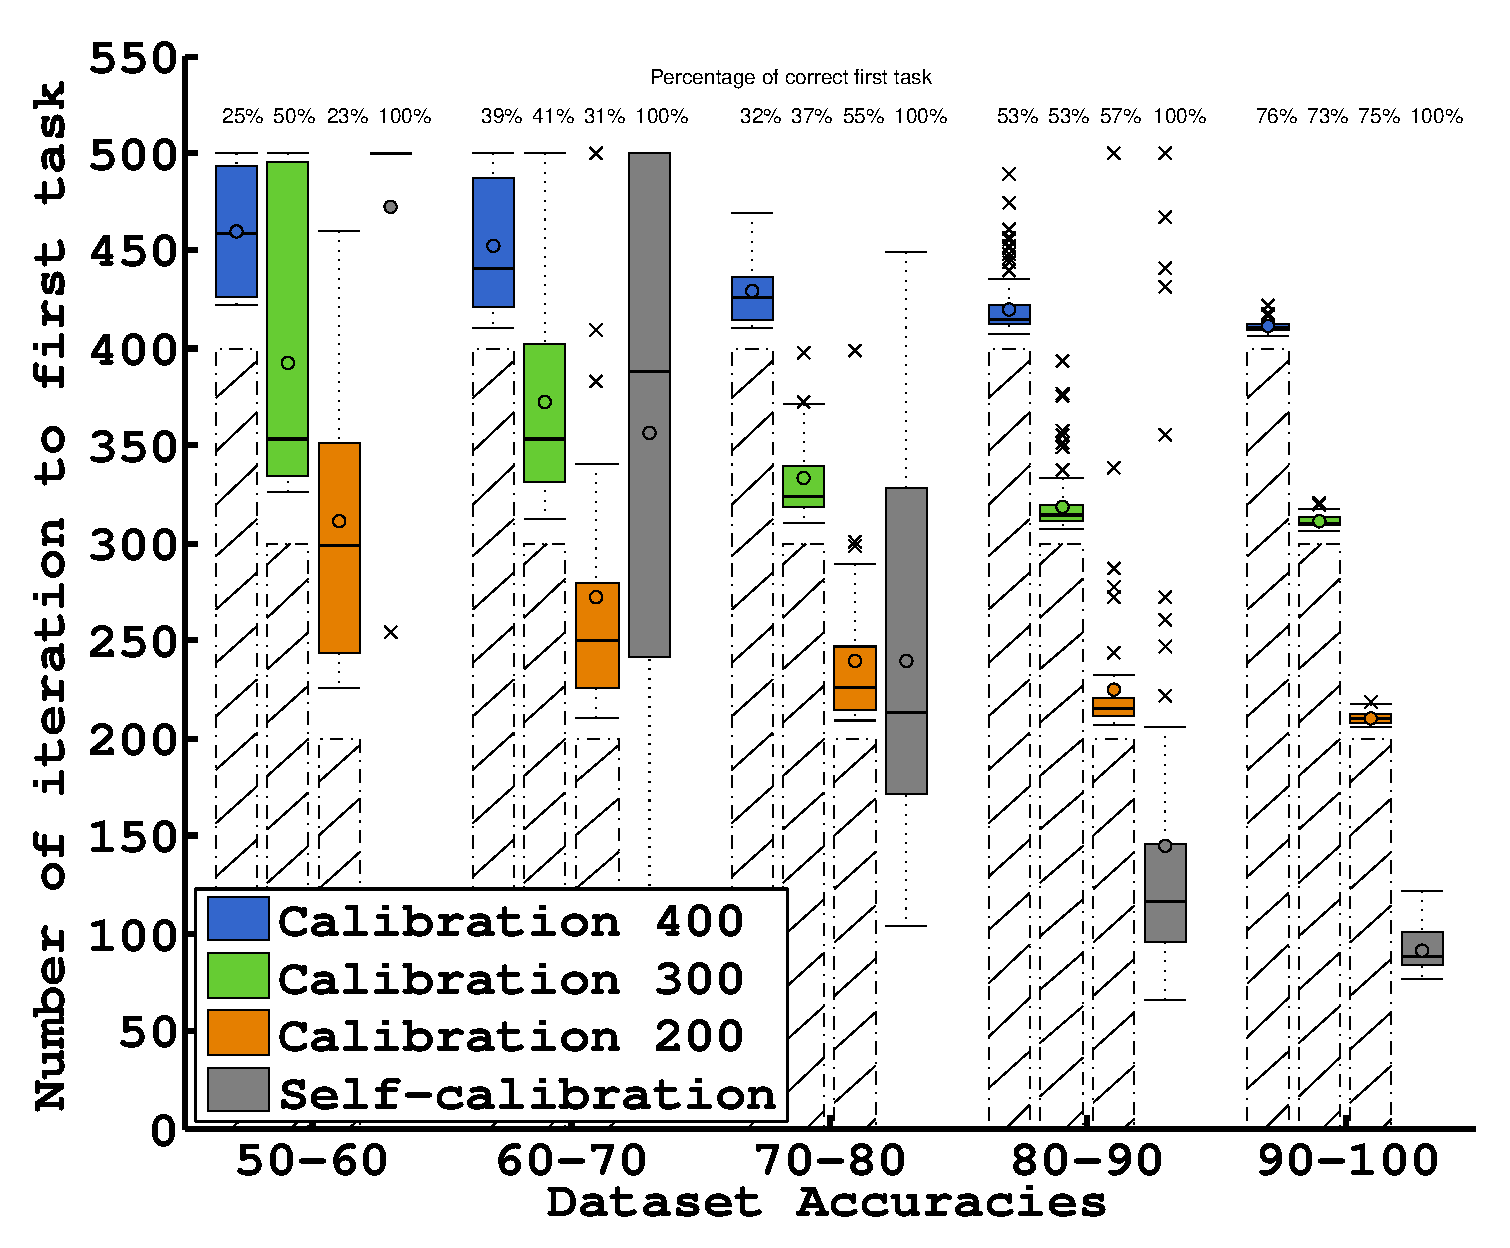
\includegraphics[width=\plotsize\columnwidth]{\imgpath/plot_EEG_calib_firstconf.eps}
\caption{Number of steps to complete first task with EEG data. The agent planned its action using our uncertainty based method. The percentage of time the task first task was correct is show on top of the each box plot. The method scale well to EEG data. For our self-calibration method, the learning time is strongly correlated with the dataset quality. Contrary to the standard calibration approaches, we do not make mistakes with low quality datasets.}
\label{fig:firstEEG}
\end{figure} 

Compared to calibration methods, our algorithm allows to complete the first task without errors. However calibration methods, which do not update their classifier once calibrated, identify more tasks incorrectly. In addition, for the calibration method, the time to first target is way less correlated to the dataset quality than our self calibration procedure. The fact of training one classifier per task makes our algorithm more robust. We will discuss potentials reasons of such errors in section~\ref{chapter:bci:cheating}.

\subsection{Cumulative performances}

Figure~\ref{fig:nCorrectEEG} compares the number of tasks that can be achieved in 500 steps. With 90\% and more dataset quality we can achieve about 20 tasks on average. The results are consistent with artificial dataset analysis.

\begin{figure}[!htbp]
\centering
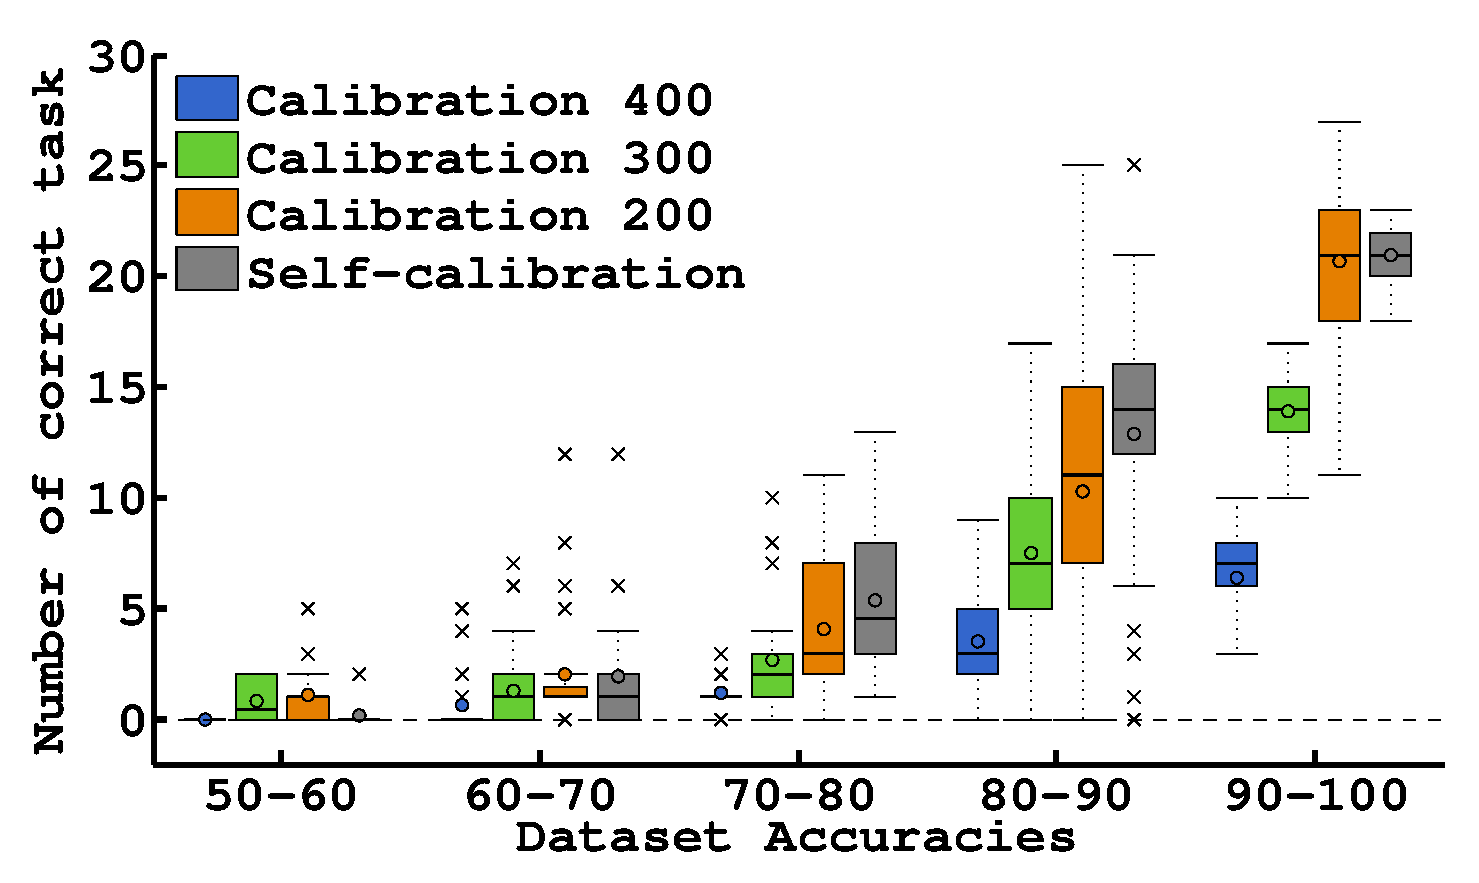
\includegraphics[width=\plotsize\columnwidth]{\imgpath/plot_EEG_calib_nCorrect.eps}
\caption{Number of task correctly achieved in 500 steps with EEG data. Calibration methods can not complete a significant number of task as most of the time is spent on calibration.}
\label{fig:nCorrectEEG}
\end{figure} 

The calibration methods can not complete many task as a significant amount of iteration was used for calibrating the system. A calibration of 200 steps makes as many good estimation than our method, but it also makes many wrong estimation, see Figure~\ref{fig:nWrongEEG}. For calibration methods, the less time spent on calibration, the poorer the classifier which implies more mistakes.

\begin{figure}[!htbp]
\centering
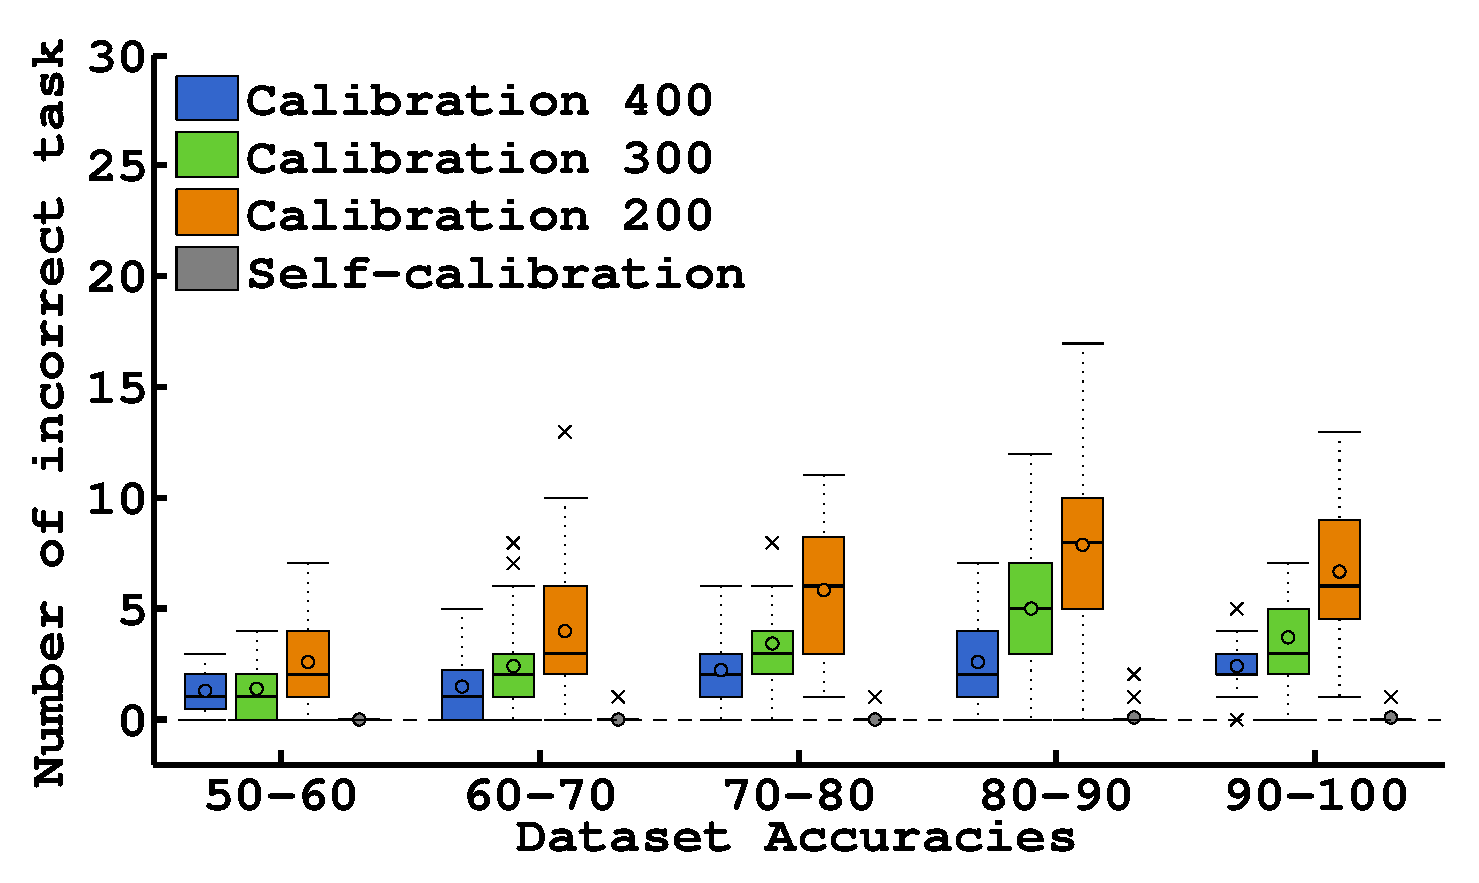
\includegraphics[width=\plotsize\columnwidth]{\imgpath/plot_EEG_calib_nWrong.eps}
\caption{Number of task incorrectly achieved in 500 steps with EEG data. Calibration methods, which do not update their models once calibrated, make more errors.}
\label{fig:nWrongEEG}
\end{figure}

\subsection{Last 100 iterations performances}

Figure~\ref{fig:nCorrectEEG_last100} compares the number of task that can be achieved during the last 100 steps with EEG data. During the last 100 steps, all method are active at their full potential as no time is lost in calibrating the system. With 80-90\% dataset quality, all methods achieve an average success rate of one task every 20 steps. However calibration methods, which do not update their models once calibrated, make more mistakes (see figure \ref{fig:nWrongEEG_last100}). While our method achieve slightly less task during the last 100 steps, it makes less mistakes, which seems to indicate our method is more conservative. We will discuss that point in section~\ref{chapter:bci:cheating}.

\begin{figure}[!htbp]
\centering
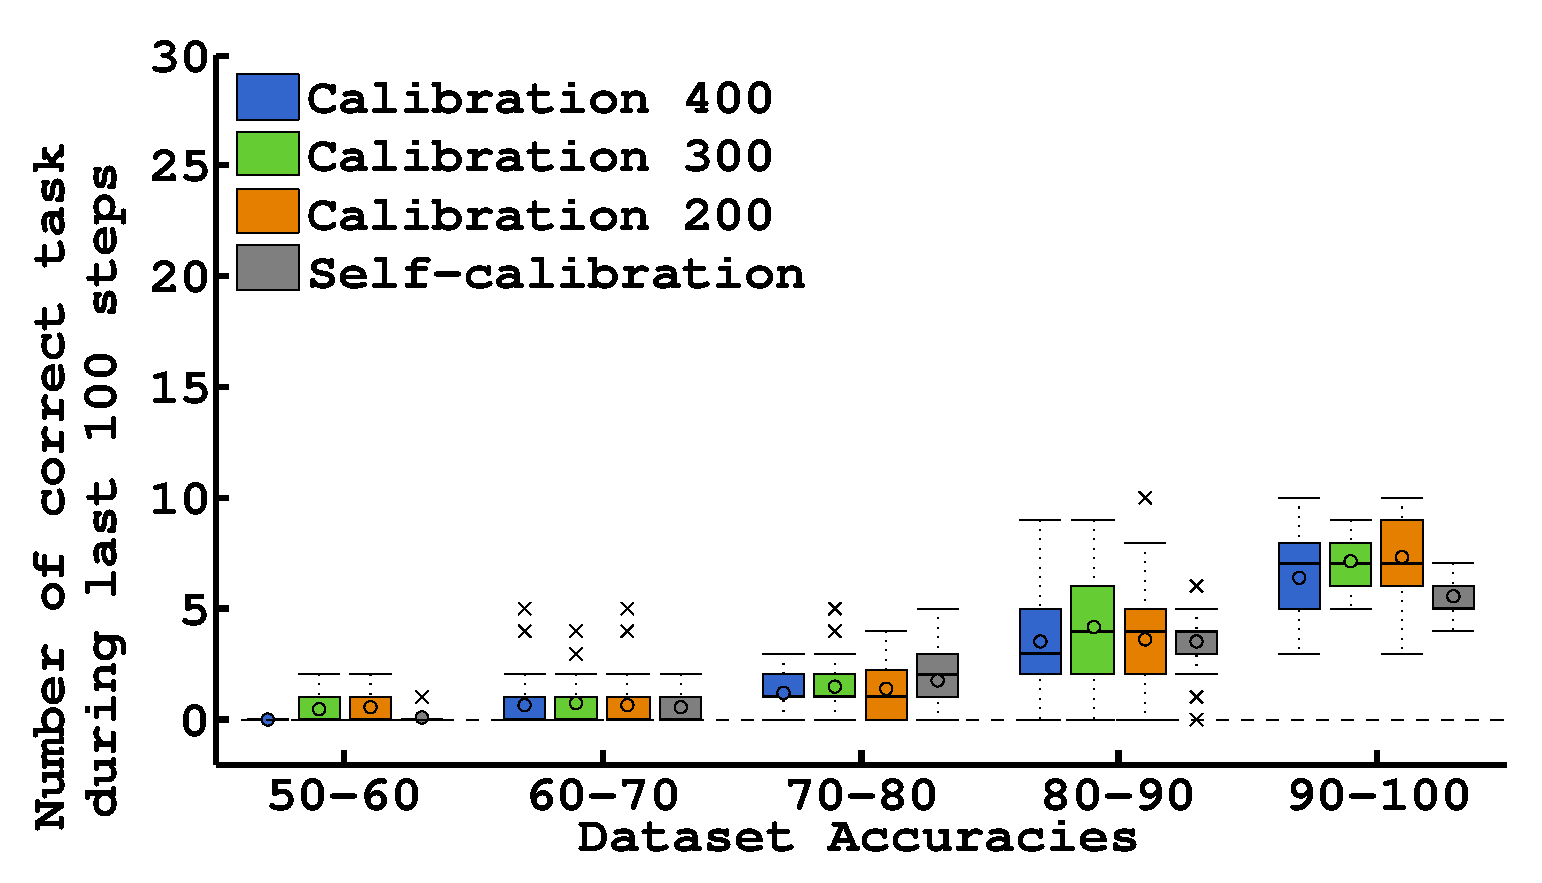
\includegraphics[width=\plotsize\columnwidth]{\imgpath/plot_EEG_calib_nCorrect_last100.eps}
\caption{Number of task correctly achieved during the last 100 steps with EEG data. All methods have equivalent successful reaching rate.}
\label{fig:nCorrectEEG_last100}
\end{figure} 

\begin{figure}[!htbp]
\centering
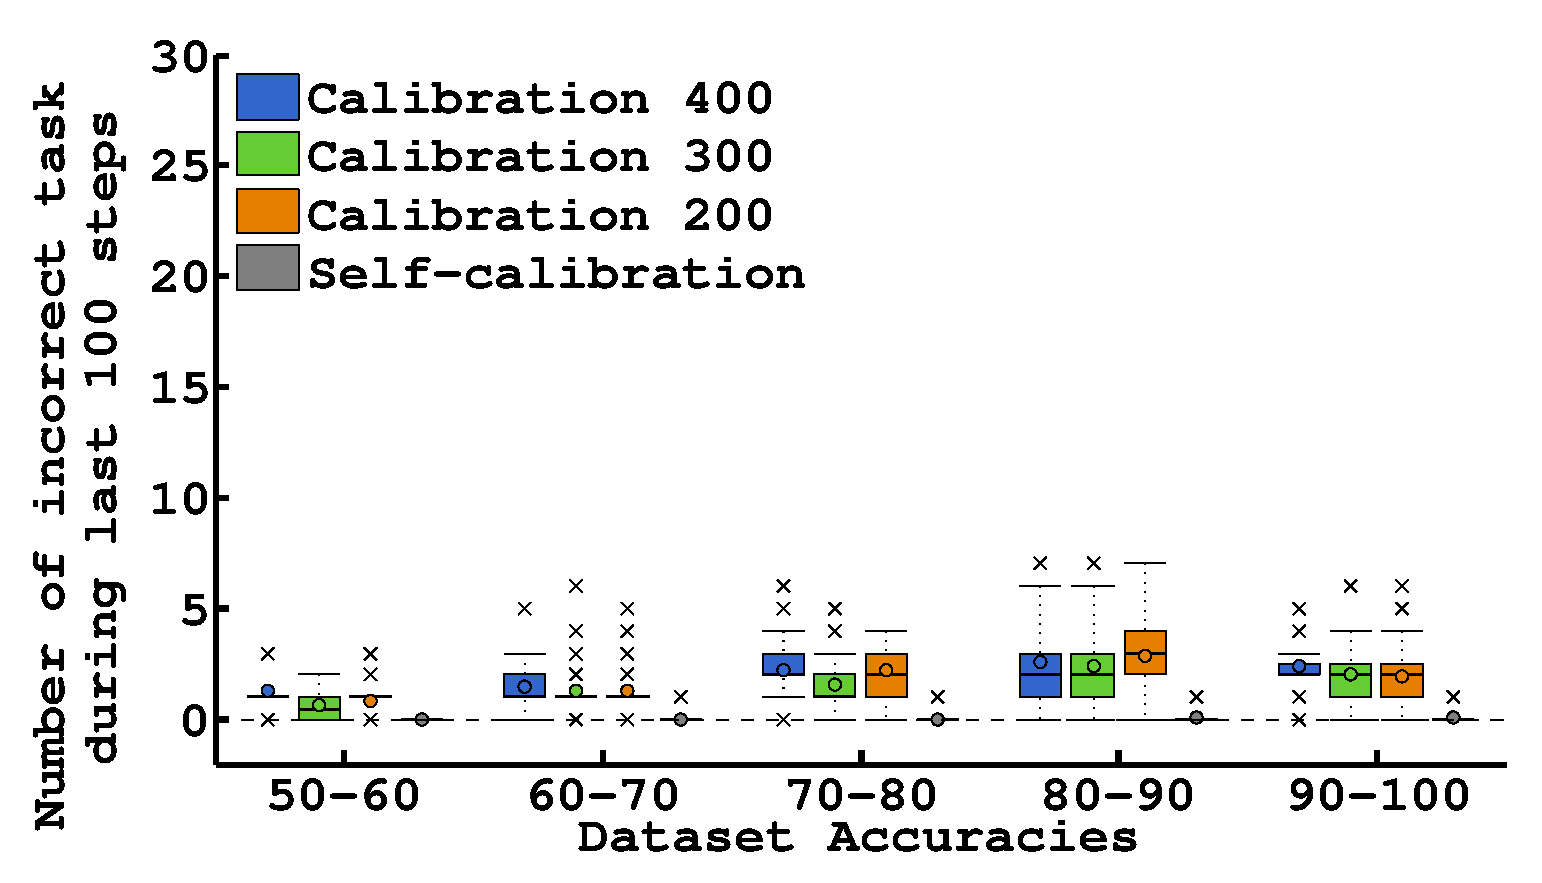
\includegraphics[width=\plotsize\columnwidth]{\imgpath/plot_EEG_calib_nWrong_last100.eps}
\caption{Number of task incorrectly achieved during the last 100 steps with EEG data. Calibration methods, which do not update their models once calibrated, make more errors.}
\label{fig:nWrongEEG_last100}
\end{figure} 

%%%%%%%%%%%%%%%%%%%%%%%%%%%%%%%%%%%%%%%%%%%%%%
%%%%%%%%%%%%%%%%%%%%%%%%%%%%%%%%%%%%%%%%%%%%%%
%%%%%%%%%%%%%%%%%%%%%%%%%%%%%%%%%%%%%%%%%%%%%%
%%%%%%%%%%%%%%%%%%%%%%%%%%%%%%%%%%%%%%%%%%%%%%
%%%%%%%%%%%%%%%%%%%%%%%%%%%%%%%%%%%%%%%%%%%%%%
\section{Why we are cheating with pre-recorder EEG samples}
\label{chapter:bci:cheating}

We can identify two main differences between our method and the usual calibration procedure for this kind of BCI experiments:
\begin{enumerate}
\item \textbf{Online update of multiple classifiers.} Our method integrates new data at every step whose label can differ between task hypothesis. For incorrect task hypothesis, the associated label can be incorrect and decrease the performance of the associated classifier. This dynamic can be observed in figure \ref{fig:sequence_evolution} where classifiers associated to incorrect tasks (in blue) have lower estimated accuracies than the correct one (in red). As a result our algorithm makes different predictions and updates for each hypothesis.
\item \textbf{Positive/Negative percent ratio of training examples}. Following the literature \cite{chavarriaga2010learning, iturrate2013task} we used a 80/20 percent ratio. Table \ref{tab:correctLabelRatio} shows the positive/negative ratio obtained following our planning method. The ratio we obtain is more balanced, resulting in classifiers with better properties. However a 50/50 percent ratio may lead to practical problems during online real world experiments and should be studied in more details.
\end{enumerate}

This latter aspect concerning the positive/negative ratio of training example is usually required due to the properties of the signal we seek for in the subjects. Indeed Errp signals are signals that corresponds more to non expected movement from the agent than to voluntary erroneous assessment. By this we mean that the user should not expect the agent o make a mistake for the signal to be present and of good intensity. This explains why, during the calibration phase of their system, researchers uses 80 percent of the time a correct action (i.e. moving towards the goal), and only 20 percent of the time an incorrect action which is therefore unexpected. This is possible because during the calibration period, both the user and the agent are aware of the target considered.

However, in our scenario, the agent is not aware of the goal the user has in mind, Therefore it is impossible to guarantee such an 80/20 percent ratio of positive/negative examples. In practice our method acquired as many correct and incorrect samples according to the true intended task, see Table~\ref{tab:correctLabelRatio}.

\begin{table}
\centering
\rowcolors{2}{gray!25}{white}
\begin{tabular}{c c c}
Dataset Accuracies & Self-calibration & Calibration \\ \hline
50-60 & 0.48 (0.02) & 0.8 (0) \\
60-70 & 0.50 (0.03) & 0.8 (0) \\
70-80 & 0.53 (0.03) & 0.8 (0) \\
80-90 & 0.57 (0.03) & 0.8 (0) \\
90-100 & 0.59 (0.01) & 0.8 (0) \\
\end{tabular}
\caption{Mean ratio of positive examples in training dataset (standard deviation shown in parenthesis). Calibration procedure for ErrP EEG signal usual account for a 80 percent ratio of positive examples. However when following our method we collect as many positive than negative examples. This is likely to impact the quality of Errp signal received from the human during online experiment.}
\label{tab:correctLabelRatio}
\end{table}

As a first observation this can explain the results of Figure~\ref{fig:firstEEG}, Figure~\ref{fig:nWrongEEG}, and Figure~\ref{fig:nWrongEEG_last100} where the calibration method, while using the exact same update equation, makes more mistakes than our self-calibration method. Apart from the fact that our method train one classifier per class, the method which calibrates using 400 examples should have similar performances than our self-calibration. But the calibration based method only observed 80 samples corresponding to the ``incorrect'' class, while the self-calibration method observed 200 in average after 400 steps. As the data are of relatively high dimension, 80 sample is not that to build a good enough model, especially for those low quality datasets.

As a results, the properties of the classifiers are different between our self-calibration method and the one from the calibration procedure. Figure~\ref{fig:calibFail} shows the difference between the perceived accuracy of the classifiers (i.e. when estimating their quality on their training data) versus the actual accuracy of the classifiers (i.e. when estimating their quality on the remaining data in our bigger dataset). For dataset of good quality, our method generates classifiers that are under-confident while the calibration method tend to produce over-confident classifiers. This over-confidence is likely to explain the high number of estimation error when relying on the  calibration procedure, versus the very low error rate observed for our self-calibration method which tend to under-estimate the quality of its classifiers.

\begin{figure}[!htbp]
\centering
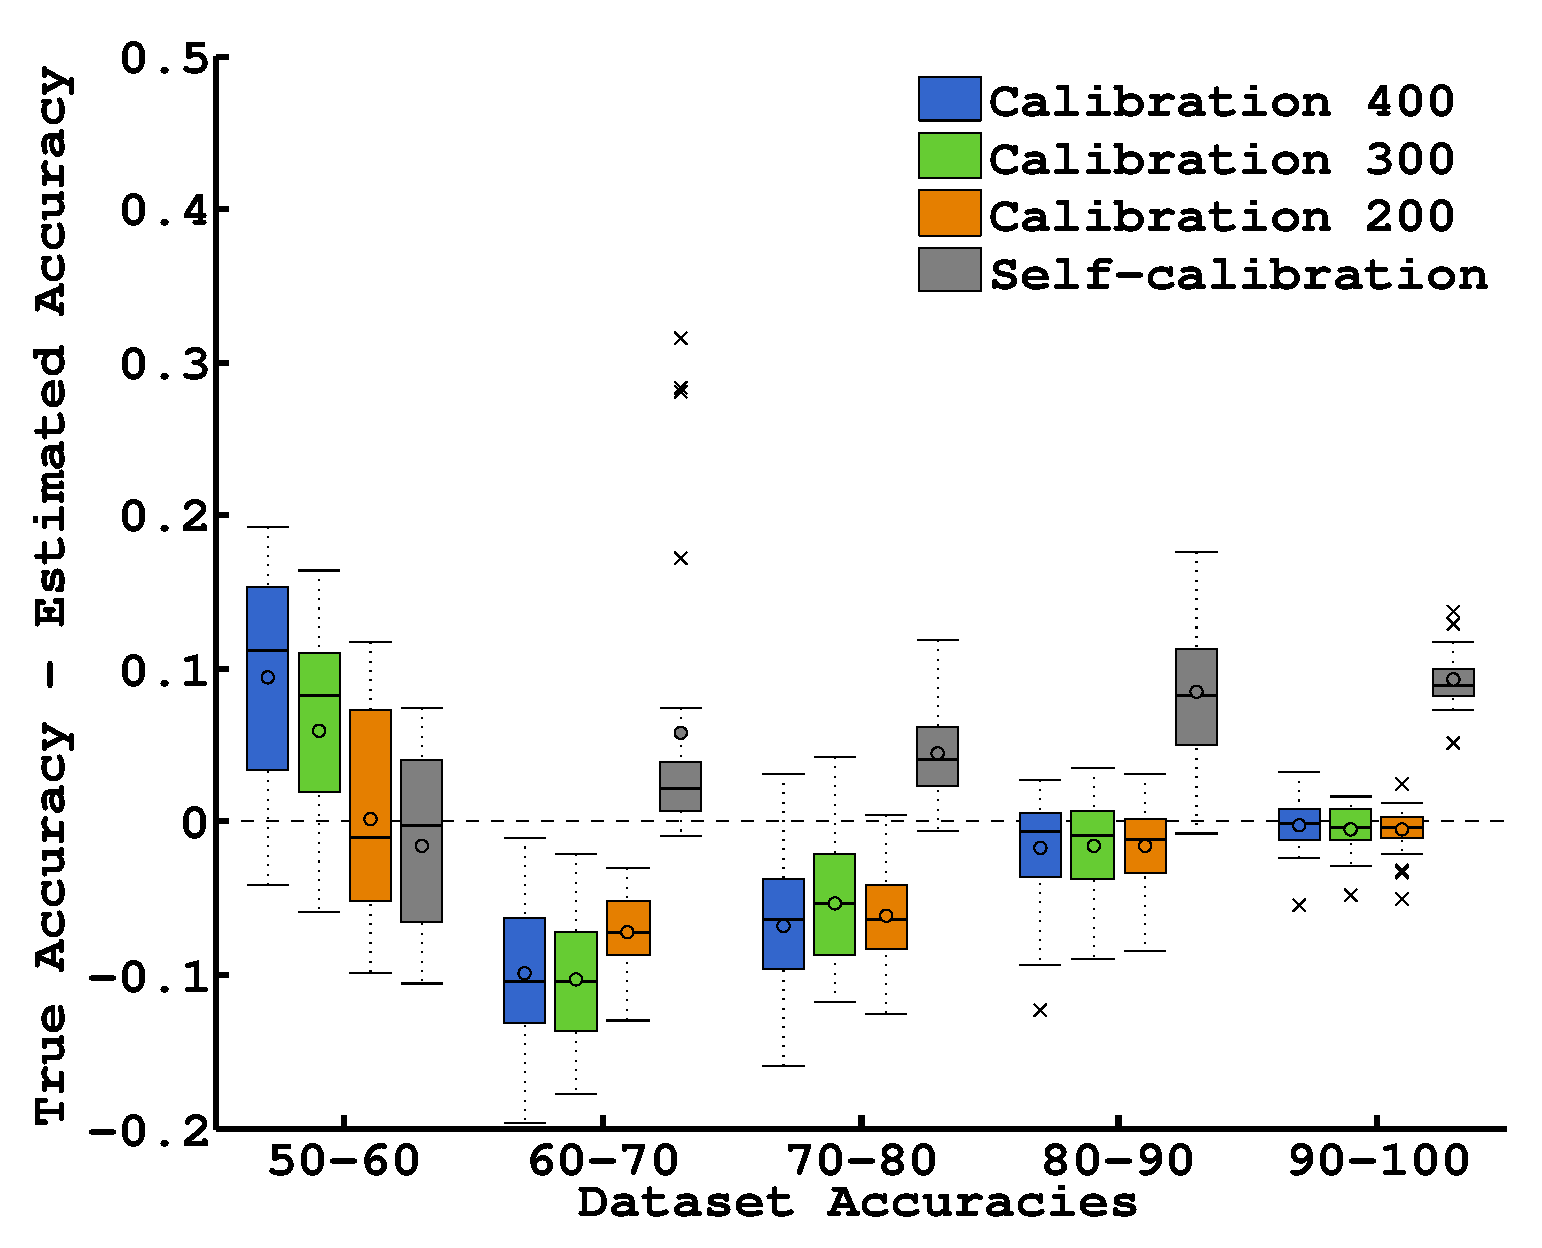
\includegraphics[width=\plotsize\columnwidth]{\imgpath/plot_explaination_for_calib_failure.eps}
\caption{Difference between true accuracy and estimated accuracy. True accuracy is the performance of the classifier on the unused data. Estimated accuracy is the 10 fold cross validation performance of the classifier on collected data. A negative(positive) value indicates the classifier is over(under)-estimating its performance. Calibration methods tend to produce over-confident classifiers, certainly due to the biased positive to negative training example ratio, see table \ref{tab:correctLabelRatio}.}
\label{fig:calibFail}
\end{figure}

But, while this conclusion seems satisfying and is likely to explain the observation made int he previous section, we forgot to considerer that the data we used in our simulated experiment where collected using an 80/20 percent ratio between the correct and incorrect signal samples. Will the brain signals conserve similar properties when using our self-calibration method, which collect samples with a 50/50 percent ratio? This is unlikely. 

The work of Chavarriaga et al. and Iturrate et al. shows that high variability in the teaching signals properties are observed when varying the task and the teaching protocol \cite{chavarriaga2010learning, iturrate2013task}. Indeed Errp signals are signals that corresponds more to non expected movement from the agent than to voluntary erroneous assessment. This means that the user should not expect the agent to make a mistake for the signal to be present and of good intensity. With a 50/50 percent ratio, the subject is unlikely to be surprise and may produce signal of lower quality.

During our first session of online experiments with real subjects we observed that the quality of the received data were very poor, even for subjects that were highly trained to assess the agent action using their brain. The main cause was the behavior of the agent which is very confusing with respect to the goal. At the beginning of the experiments, for the subject the agent seems to act randomly, without trying to move toward the target. Therefore subject have high difficulty to generated Errp signals of good quality, which makes the process longer, do not improve the behavior of the agent and further reduces the engagement of the users in the teaching task. Studying in more details the impact of the agent behavior on the Errp signals is not our main goal and more thorough analysis is required to provide more firm conclusion.

Consequently, while some subject succeeded in the teaching task, we observed a relatively high number of errors and long teaching time. Therefore we decided to include an a priori information in the system in order to improve the learning time and the behavior of the agent. This properties relates to difference in power (sum of the EEG feature squared) between EEG signals of meaning ``correct'' and ``incorrect''. The signal related to the unexpected, erroneous action, being more powerful. However this property is not enough to identify with certainty ``correct'' and ``incorrect'' signals. In next section, we study in more detailed this properties and show how it can be exploited in our system.

%%%%%%%%%%%%%%%%%%%%%%%%%%%%%%%%%%%%%%%%%%%%%%
%%%%%%%%%%%%%%%%%%%%%%%%%%%%%%%%%%%%%%%%%%%%%%
%%%%%%%%%%%%%%%%%%%%%%%%%%%%%%%%%%%%%%%%%%%%%%
%%%%%%%%%%%%%%%%%%%%%%%%%%%%%%%%%%%%%%%%%%%%%%
%%%%%%%%%%%%%%%%%%%%%%%%%%%%%%%%%%%%%%%%%%%%%%
\section{Including Prior Information}
\label{chapter:bci:priorpower}

In this section we detail how we can exploit the difference of power between our two class of signals. The signal related to the unexpected, erroneous action, being more powerful, it gives an an absolute information about which group of point should mean ``incorrect''. While this property is not enough to identify with certainty ``correct'' and ``incorrect'' signals, we will see that it allow to differentiate between symmetric hypothesis, which improves the performances of our algorithm as well as the behavior of the agent at run time.

\subsection{Difference of power between correct and incorrect signal}

As shown in Figure~\ref{fig:EEGsample}, the EEG signals associated to ``incorrect'' labels have slightly more amplitude than the one associated to ``correct'' labels, especially at around 300ms.

\begin{figure}[!htbp]
\centering
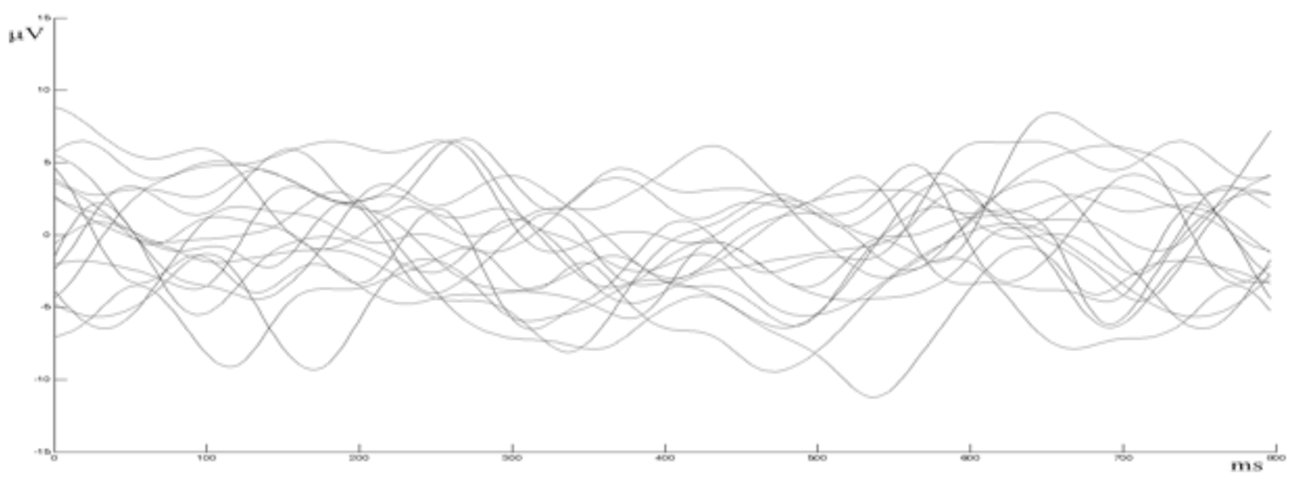
\includegraphics[width=\eegsize\columnwidth]{\imgpath/illustration/correctEEG.pdf}
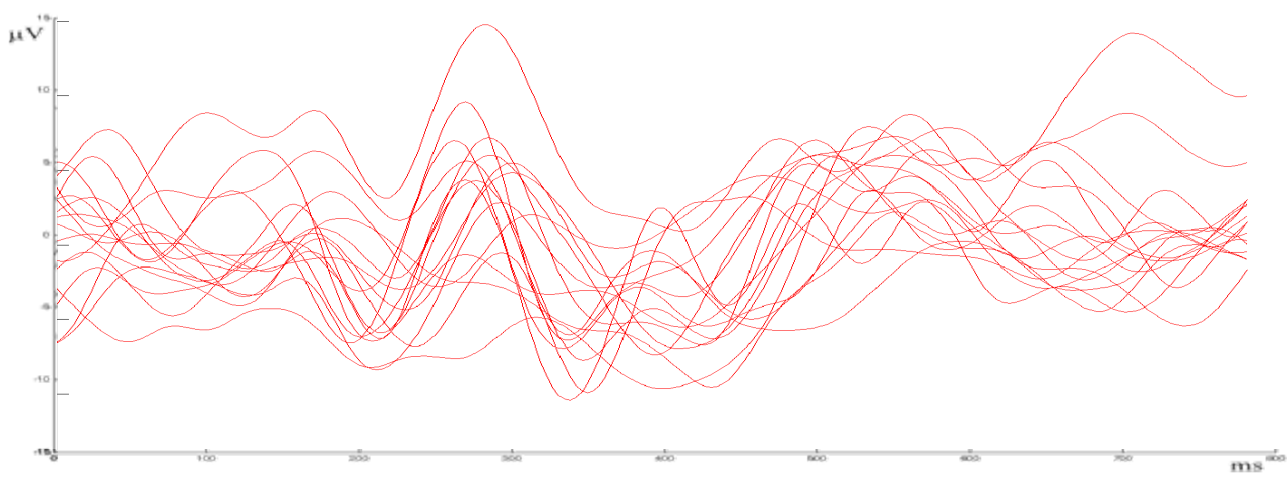
\includegraphics[width=\eegsize\columnwidth]{\imgpath/illustration/errorEEG.pdf}
\caption{Low-pass filtered EEG signals associated to ``correct'' labels (top) and to ``incorrect'' labels (bottom).  The signals have slightly different amplitudes, especially at around 300ms. \todo{change with one figure inkscaped}}
\label{fig:EEGsample}
\end{figure}

To build our feature vector we consider two fronto-central channels (FCz and Cz) in a time window of $[200,700]$ ms (being 0 ms the action onset of the agent) and downsampled the signal to $32$ Hz. Each element of the feature vector is the value in microvolts of the signal at the corresponding time. To compute the power information contained in our signal we simply compute the sum of the square of each feature representing our signal. This simple approximation allows to capture the slight difference in power between ``incorrect'' and ``correct'' signals (see Figure~\ref{fig:EEGpower}). However this is not enough to classify a single signal with more than 60 percent accuracy, which is almost random. But considering a group of point we can observe that the mean of power of the ``incorrect'' class is higher that the mean power of the ``correct'' class. We will exploit this property as an a priori information of which group of point should means ``correct'' or ``incorrect''.

\begin{figure}[!htbp]
\centering
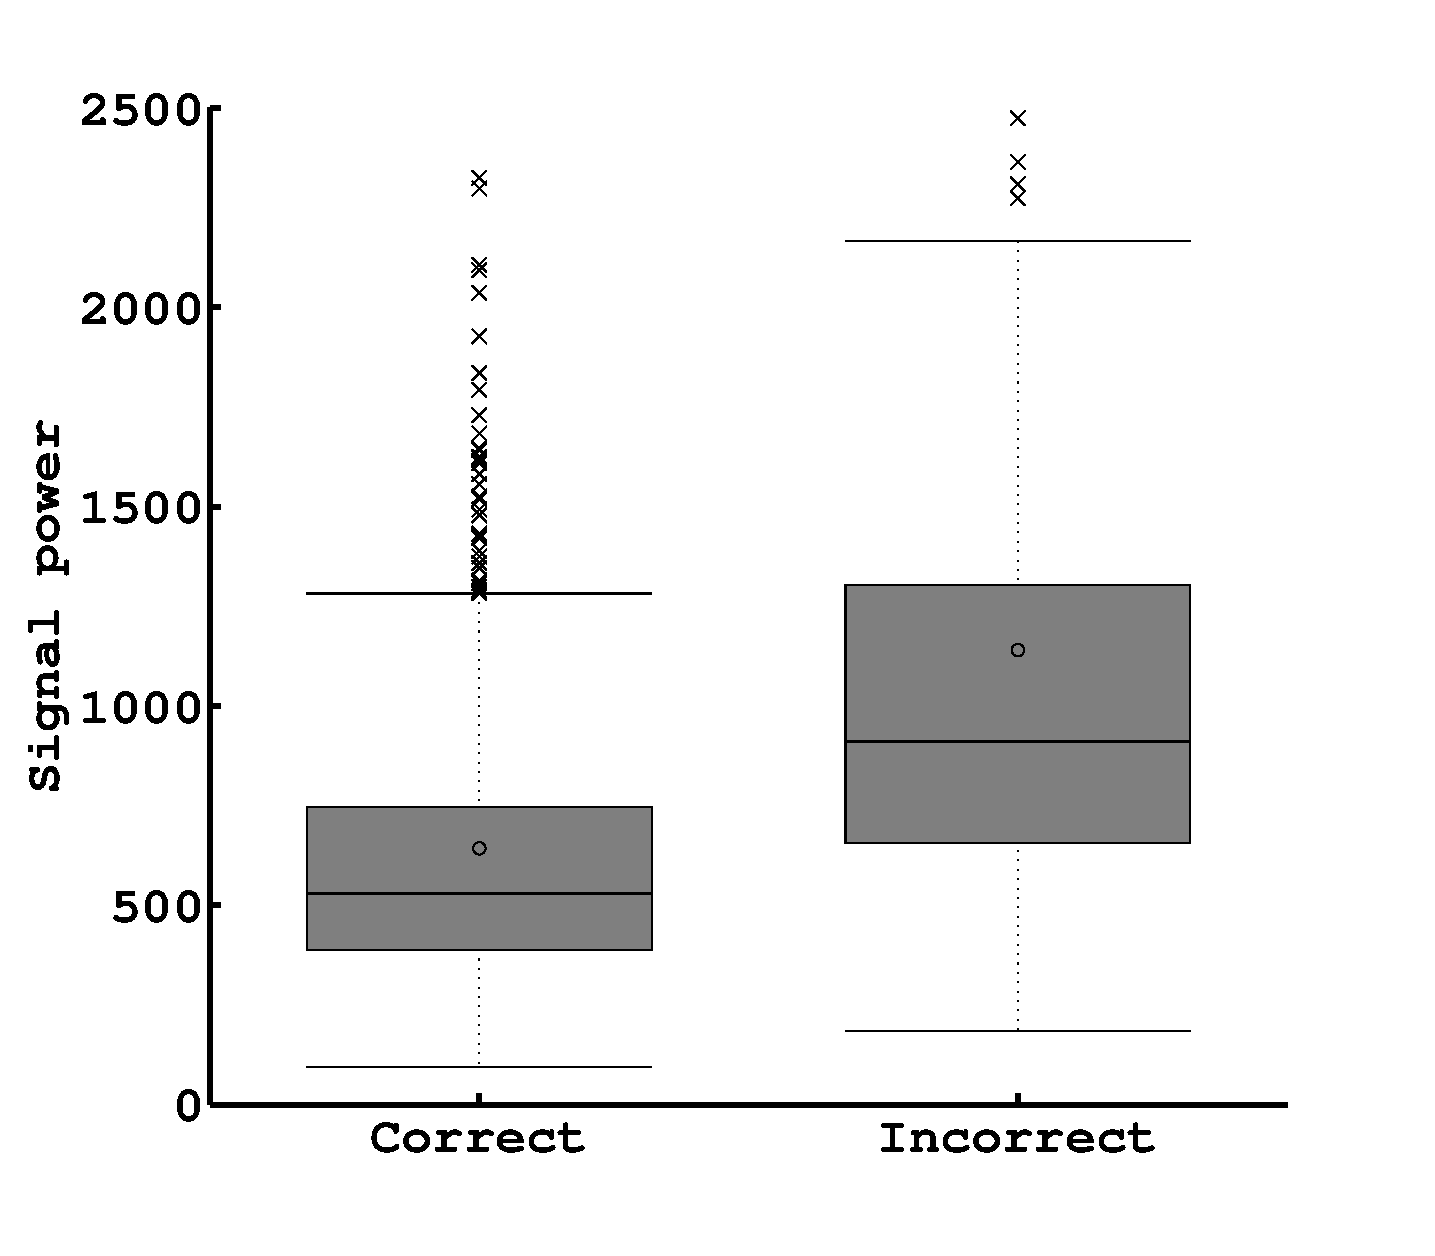
\includegraphics[width=\plotsize\columnwidth]{\imgpath/powermatching/powerdiff.eps}
\caption{Box plot of the power of each individual signal for one of our EEG dataset. The datasetis of good quality and our classifier reaches a classifiaction rate of 83 percent. The mean power information from the ``incorrect'' signals is higher than for the ``correct'' ones.}
\label{fig:EEGpower}
\end{figure} 


To compute the power information of signal associated to the ``correct'' labels, we simply compute the weighted mean of the power of the signals weighted by their probability of being of label ``correct''. 
\begin{eqnarray}
powerCorrect(\xi_t) = \frac{\sum_{i = 1}^{M} p(l^c = ``correct"| e_i , \theta) ~~ e_i^T e_i}{\sum_{i = 1}^{M} p(l^c = ``correct"| e_i , \theta)}
\label{eq:powerCorrect}
\end{eqnarray}
with $\theta$ representing the classifier trained on the available signal-label pairs associated to the task $\xi_t$.

Similarly for the ``incorrect'' labels, we simply compute the weighted mean of the power of our signals weighted by their probability of being of label ``incorrect''. 
\begin{eqnarray}
powerIncorrect(\xi_t) = \frac{\sum_{i = 1}^{M} p(l^c = ``incorrect"| e_i , \theta) ~~ e_i^T e_i}{\sum_{i = 1}^{M} p(l^c = ``incorrect"| e_i , \theta)}
\label{eq:powerIncorrect}
\end{eqnarray}
with $\theta$ representing the classifier trained on the available signal-label pairs associated to the task $\xi_t$.

For the dataset shown in Figure~\ref{fig:EEGpower}, the $powerCorrect = 670$ and $powerIncorrect = 1031$. Note that this is different form the value shown by the gray circle in Figure~\ref{fig:EEGpower}. For our estimate we use the probability of each point of being of one label predicted by our classifier and not the one given in input to the classifier. 

\subsection{How to use the power information}

As for the case of known signals described in chapter~\ref{chapter:lfui:known}, we will define a specific likelihood function for the information provided by the power information and combined it with the information from our initial algorithm. We define as likelihood the ratio of the power associated to the ``incorrect'' class over the one from the ``correct'' class:

\begin{eqnarray}
\L_{power}(\xi_t) = \frac{powerIncorrect(\xi_t)}{powerCorrect(\xi_t)}
\label{eq:power}
\end{eqnarray}

For our previous example of Figure~\ref{fig:EEGpower}, this ratio equals 1.54. A likelihood above 1 indicates the labels are more likely to be correctly associated with the signals. Considering now our algorithm that assign different labels for each task hypothesis and the specific case of our symmetry problems discussed in chapter~\ref{chapter:lfui:symmetries}. In such cases the correct hypothesis will have this ratio of 1.54 as the label for ``incorrect'' are actually associated to the ``incorrect'' signals. But for the symmetric case, while our non-informed algorithm could not make the difference, our new measure gives a power ratio of 0.65. Indeed as the labels are switched, the power of class ``correct'' will be higher than the one from class ``incorrect''. Now considering an other hypothesis, whose labels are fully mixed, the power ratio will be equal to 1, as point with low and high power will be equally distributed. However in this case our non-informed algorithm will be able to measure the change in classifier quality, which, for one of our test move from 83 percent to 61 percent classification rate.

Measuring the ratio of power allow to not be dependent on arbitrary absolute difference between the power values which may differ between individuals. Indeed, it would be impossible to define an absolute threshold between the power of each classes that would decide whether one task is the correct one for everyone. 

Also, we only want to measure to which extend we are associating the labels in the correct way to disambiguate between symmetric case. This is likely to improve the behavior of the agent, therefore improving the quality of the signals receive from the subjects. 

It is of crucial importance to understand the use of the power information is only possible thanks to the specific nature of the Errp EEG signals. It would be of not use for our artificial 2D datasets. However other signals may have similar properties, such as the tone of voice that could differ between ``correct'' and ``incorrect'' feedback.

Our likelihood based on the likelihood between the power component of each classes will be used as for known button as described in chapter~\ref{chapter:lfui:known}. Before running new online EEG experiments with human subjects, we verify how this new method behaves with our pre-recorded dataset. In next section, we compared the performance between using only the power information, only our initial algorithm, or the combination of both.

\subsection{Comparison with and without the power information}

We consider the same setting as for the experiments described in section~\ref{chapter:bci:EEGsignals}. 

\paragraph{Time to first task} Figure~\ref{fig:timefirst_powermatching} compares the number of iterations needed to identify the first time with confidence between our general method (matching), or using the information that ``incorrect'' signals are more powerful than the ``correct'' (power), or both method combined (power matching). The use of the power information affects the performances for the low quality dataset. For datasets of low quality, while the time to first seems more advantageous for the method using the power information, most of the estimated task are erroneous (see Figure~\ref{tab:errorTaskRatio}) which makes the use of the power information critical for such low quality data. However those errors occurs for very low quality datasets, which are not the main target of our algorithm. For such data it would be better to change the representation of the signal or the classifier used. For the datasets of higher quality, the power information allow to slightly speed up the learning compared to our method (matching) which do not rely on known information. 

\begin{figure}[!htbp]
\centering
\includegraphics[width=\plotsize\columnwidth]{\imgpath/powermatching/timefirst.eps}
\caption{Number of steps to complete first task with EEG data. Comparison between our general method (matching), or using the information that ``incorrect'' signals are more powerful than the ``correct'' (power), or both method combined (power matching). The use of the power information affects the performance for the low quality dataset. For datasets of low quality, while the time to first seems more advantageous for the method using the power information, most of the estimated task are erroneous (see Figure~\ref{tab:errorTaskRatio}) which makes the use of the power information critical for such low quality data. However those errors occurs for very low quality datasets, which are not the main target of our algorithm. For the datasets of higher quality, the power information allow to slightly speed up the learning compared to our method (matching) which do not rely on known information.}
\label{fig:timefirst_powermatching}
\end{figure} 

\begin{table}
\centering
\rowcolors{2}{gray!25}{white}
\begin{tabular}{c c c c}
    Dataset Accuracies & Matching & Power & Power-Matching \\ \hline
    50-60 & 0 & 0.83 & 0.62 \\ 
    60-70 & 0 & 0.10 & 0.02 \\
    70-80 & 0 & 0.03 & 0.03 \\
    80-90 & 0 & 0.03 & 0.02 \\
    90-100 & 0 & 0 & 0 \\
\end{tabular}
\caption{Percentage of time the first task estimated was erroneous using EEG data. Comparison between our general method (matching), or using the information that ``incorrect'' signals are more powerful than the ``correct'' (power), or both method combined (power matching). For very low quality datasets, the power information increases the number of erroneous estimation.}
\label{tab:errorTaskRatio}
\end{table}


\paragraph{Number of tasks achieved in 500 steps}

We compare the number of task correctly (Figure~\ref{fig:nCorrect_powermatching}) and incorrectly (Figure~\ref{fig:nWrongEEG_powermatching})reached in 500 steps between our general method (matching), or using the information that ``incorrect'' signals are more powerful than the ``correct'' (power), or both method combined (power matching). The power information makes more mistakes for low quality dataset which also impact the power matching method. However those errors occurs for very low quality datasets, which are not the main targets of our algorithm. For signals of above 60 percent classification rate, the power information improve the number of task we can reach. 

\begin{figure}[!htbp]
\centering
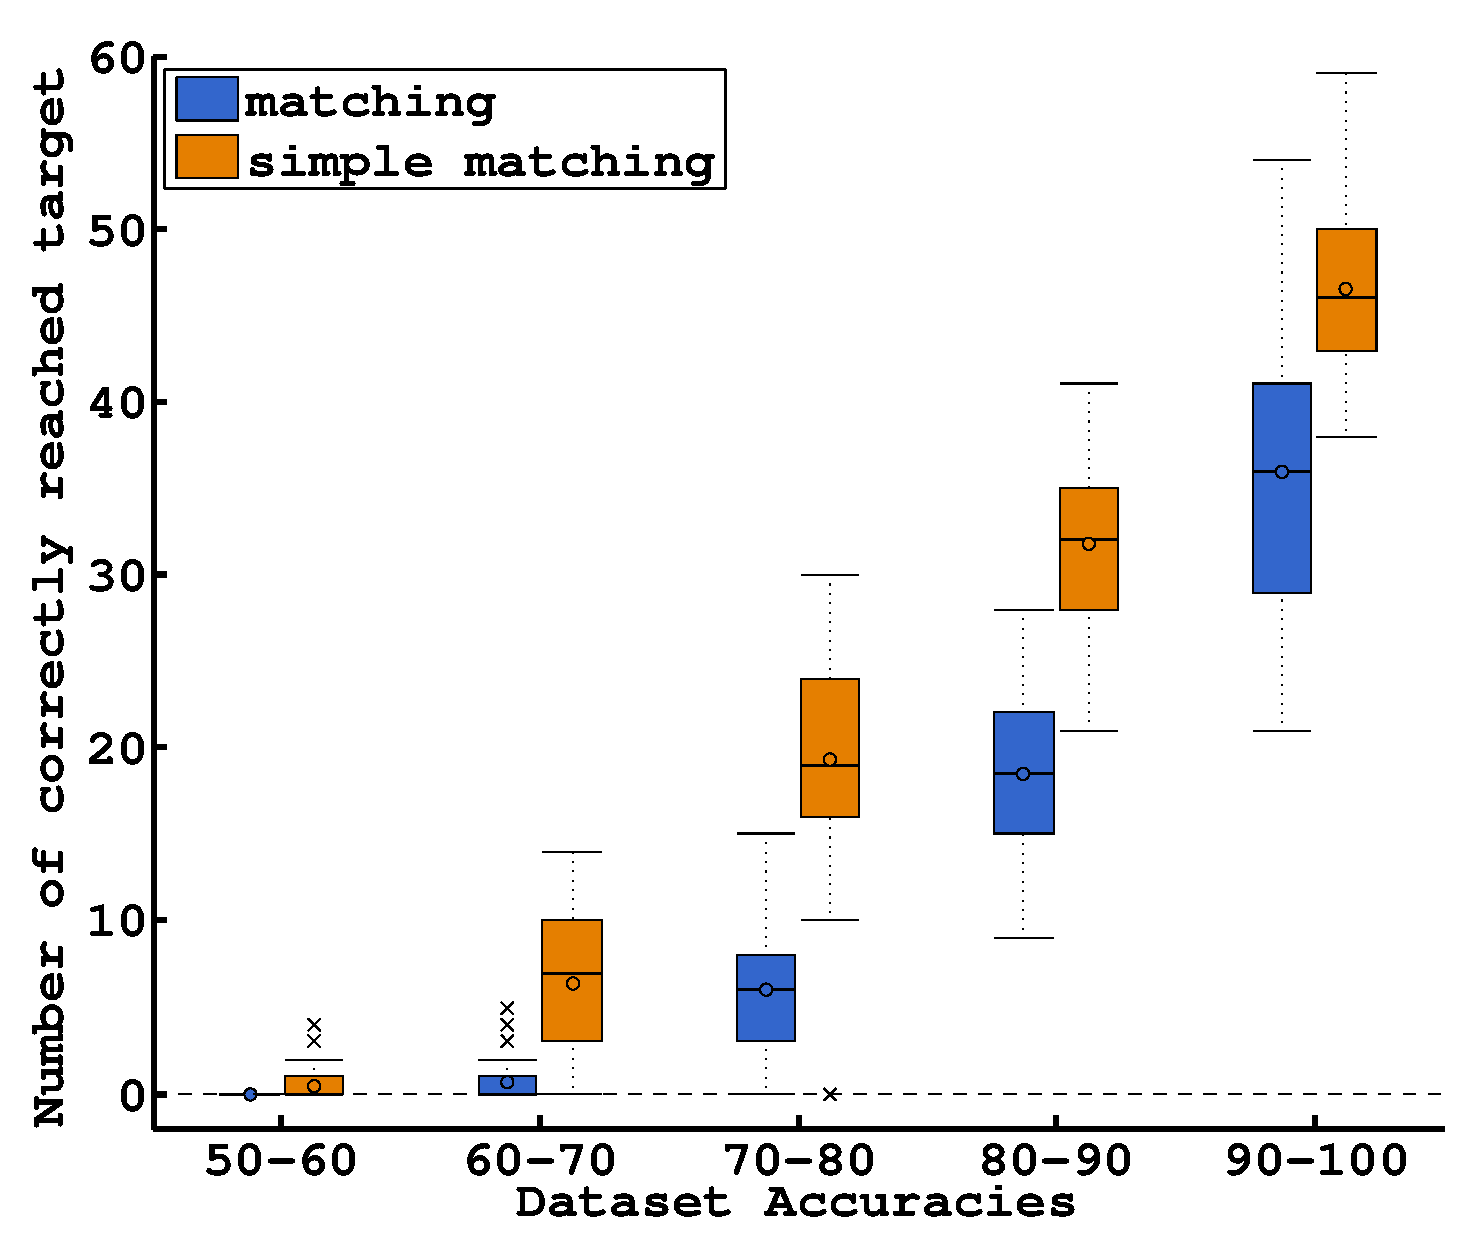
\includegraphics[width=\plotsize\columnwidth]{\imgpath/powermatching/correct.eps}
\caption{Number of task correctly achieved in 500 steps with EEG data. Comparison between our general method (matching), or using the information that ``incorrect'' signals are more powerful than the ``correct'' (power), or both method combined (power matching). The power information alone is sufficient to solve our problem but is less efficient than the other methods.}
\label{fig:nCorrect_powermatching}
\end{figure} 

\begin{figure}[!htbp]
\centering
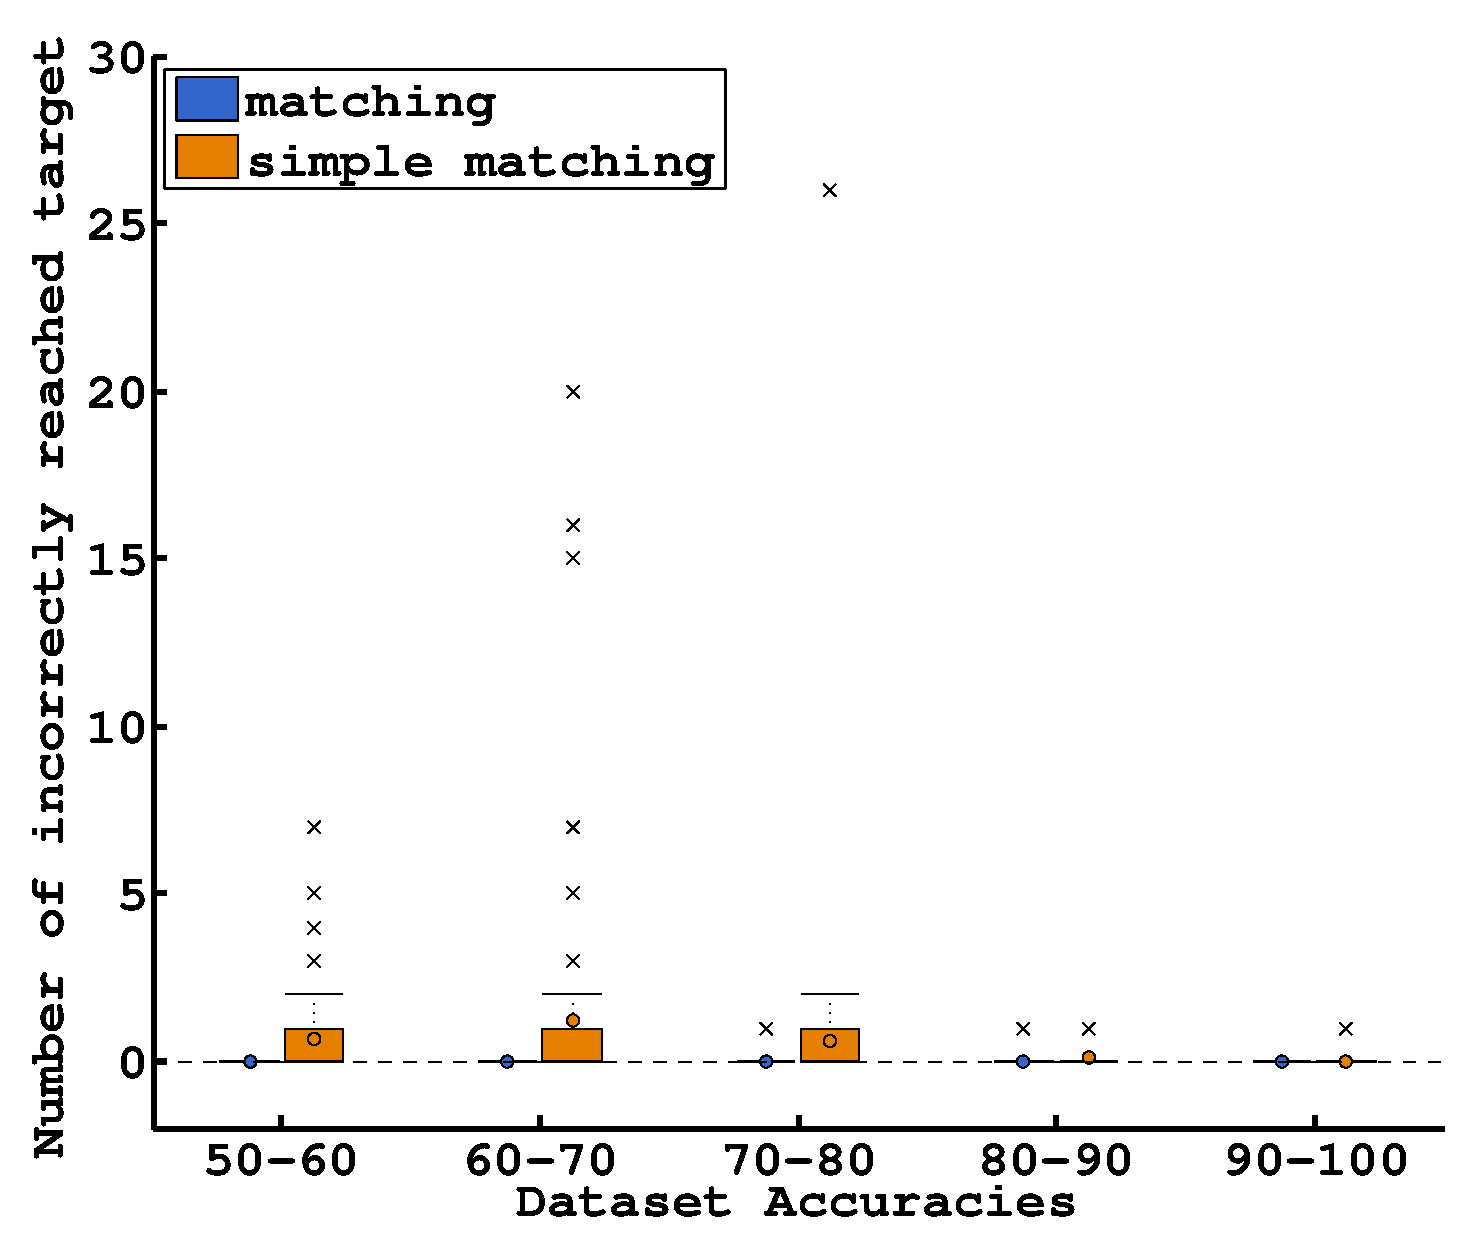
\includegraphics[width=\plotsize\columnwidth]{\imgpath/powermatching/error.eps}
\caption{Number of task incorrectly achieved in 500 steps with EEG data. Comparison between our general method (matching), or using the information that ``incorrect'' signals are more powerful than the ``correct'' (power), or both method combined (power matching). The power information makes more mistakes for low quality dataset which also impact the power matching method. However those errors occurs for very low quality datasets, which are not the main targets of our algorithm.}
\label{fig:nWrongEEG_powermatching}
\end{figure} 


The power information alone is not enough to identify a high number of task, even if the number of steps to reach the first target are similar. The difference lies in the reallocation of labels we performed after a task is identified. As described in chapter~\ref{chapter:lfui:tasttotask}, once one task is identified with confidence we propagates its labels to all the other hypothesis. As a consequence, a majority of signal have identical labels, and the number of new signals with different labels needed to pull apart two hypothesis in terms of power ratio between classes increases. This is a problem resulting in measure relying only on global measure on the data. Our non-informed method (matching), measure the global quality of each classifiers but also consider the classification of each new signals individually, which speeds up the task reaching rate as the interaction goes on. See also the discussion of Figure~\ref{fig:sequence_evolution}.


Our results confirms that the use of the power information improves the performance of our algorithm. In addition, by disambiguating faster the task with symmetric properties, it also improves the visual impression our subjects get from the behavior of the agent with improved the quality of the signals received during our experimental test. At the time of writing those lines, this study was not over and this particular point requires a more detailed analysis to show and quantify this difference. It is particularly difficult to find a measure of perception of the agent behavior to quantify the difference between the use or not of the power information. We can only report here our experience from running the experiments, which is the reason of using the power information.

%%%%%%%%%%%%%%%%%%%%%%%%%%%%%%%%%%%%%%%%%%%%%%
%%%%%%%%%%%%%%%%%%%%%%%%%%%%%%%%%%%%%%%%%%%%%%
%%%%%%%%%%%%%%%%%%%%%%%%%%%%%%%%%%%%%%%%%%%%%%
%%%%%%%%%%%%%%%%%%%%%%%%%%%%%%%%%%%%%%%%%%%%%%
%%%%%%%%%%%%%%%%%%%%%%%%%%%%%%%%%%%%%%%%%%%%%%
\section{Experiments with real users}

\begin{figure}[!htbp]
\centering
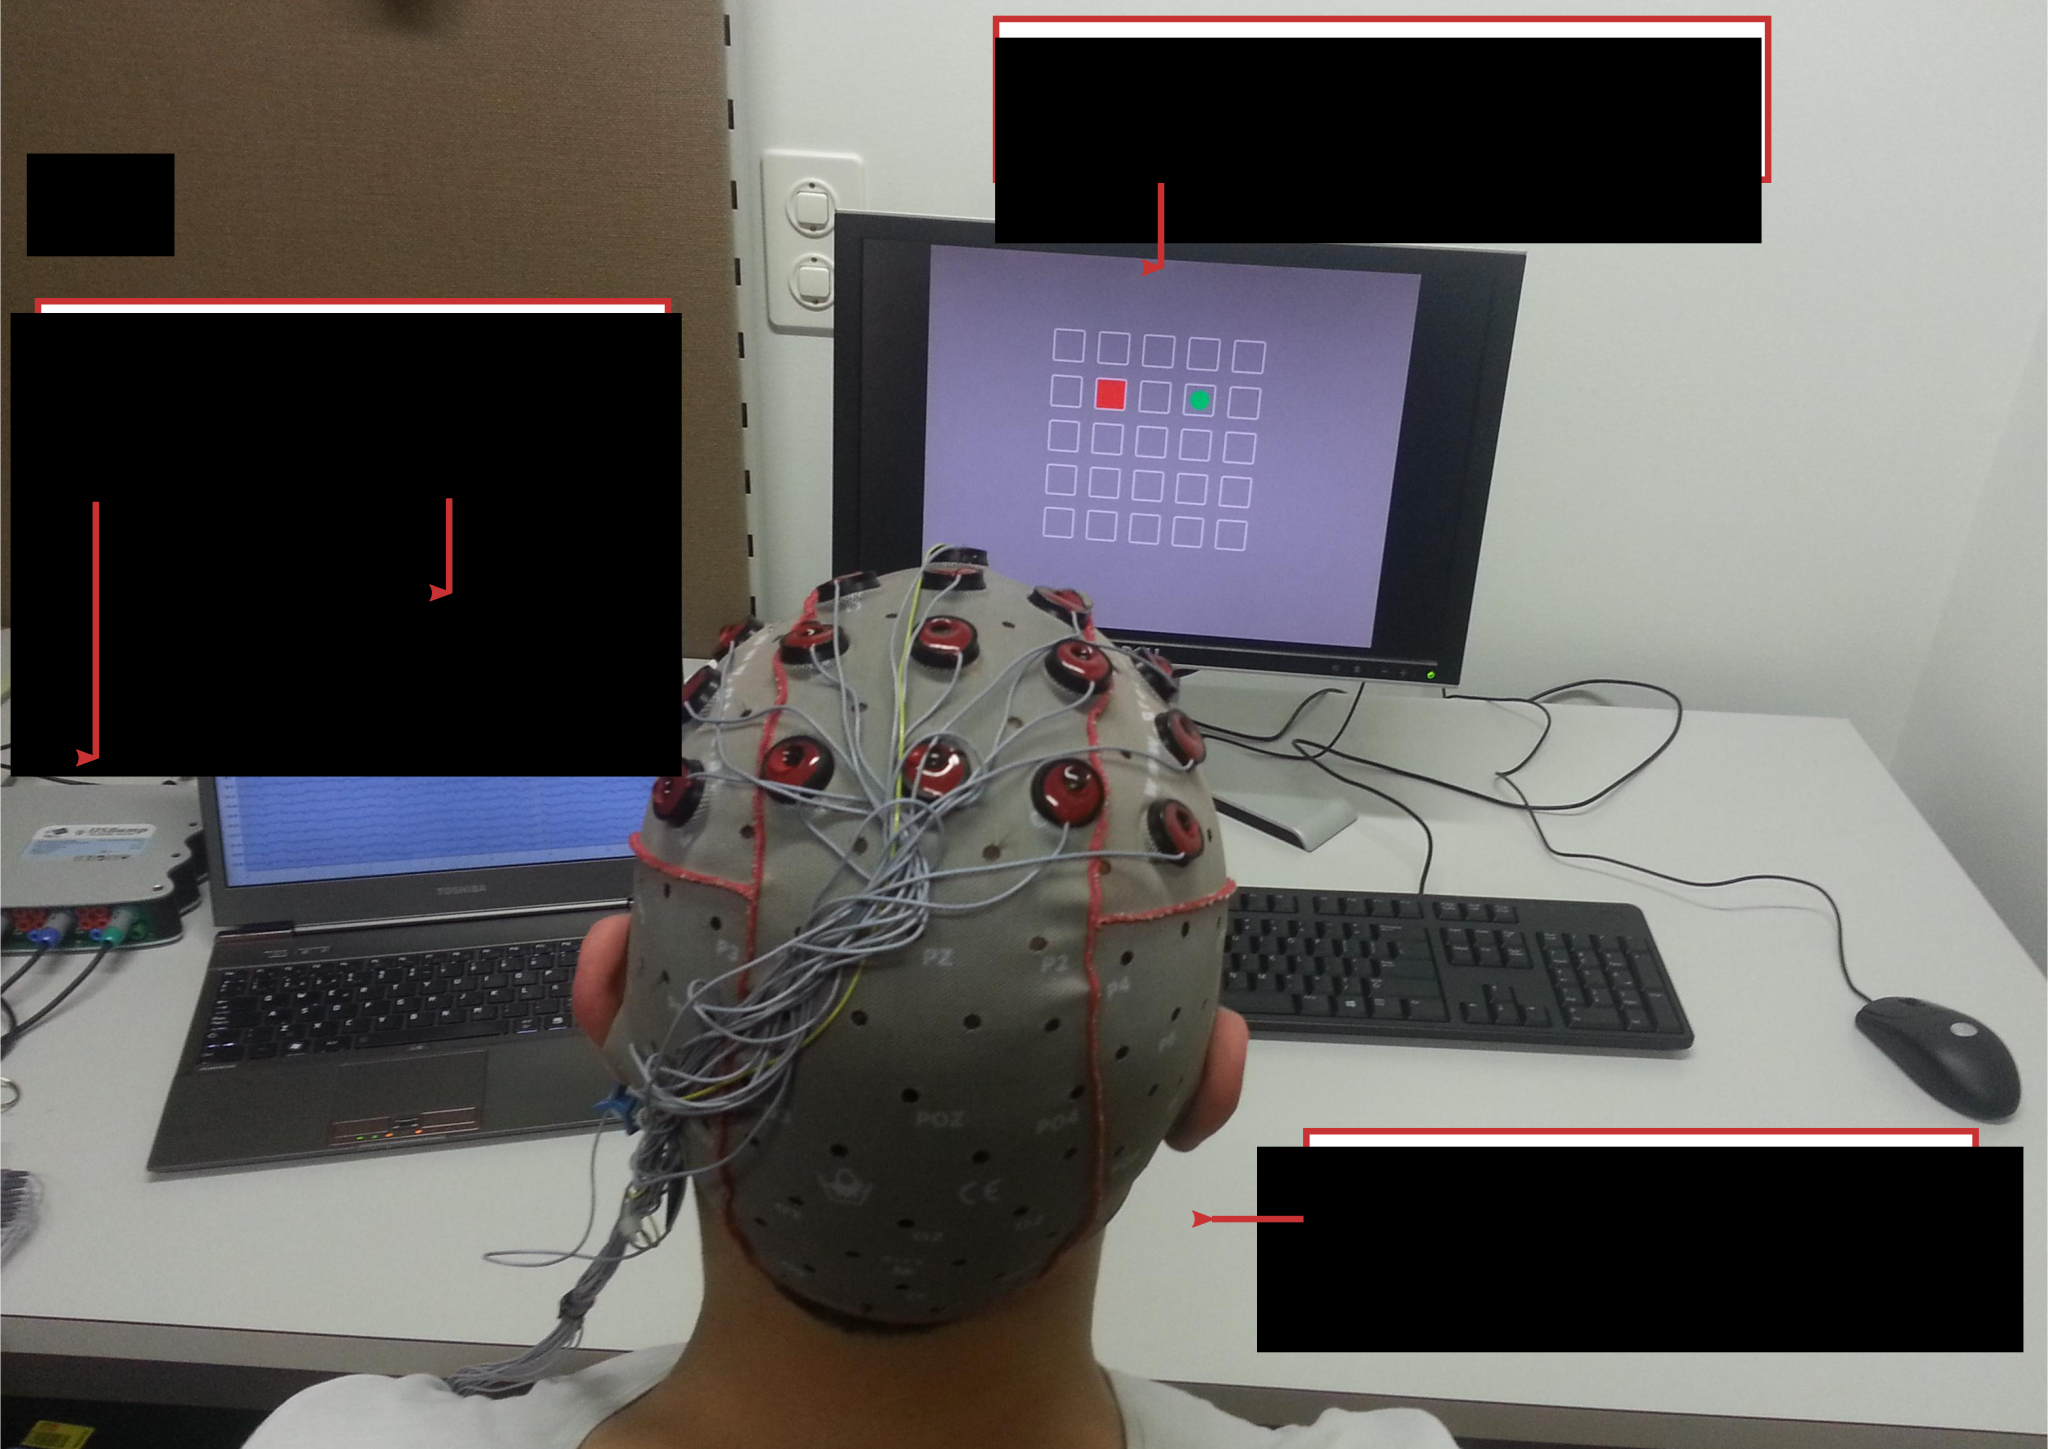
\includegraphics[width=\bcisetupsize\columnwidth]{\visualspdf/onlineXP/setup.pdf}
\caption{The BCI setup for online experiment. ON the screen is displayed the grid world with the agent in green. We displayed the intended target in red, which was selected randomly. The purpose of this red square is to help the user remembering the target and our algorithm is at no point aware of the position of this red square.}
\label{fig:BCIsetup}
\end{figure}

We ran online experiment where 3 subjects  control our agent in a virtual world. The setup of our online experiment is shown in Figure~\ref{fig:BCIsetup}. Each subject was asked to mentally assess the agent's actions with respect to a given target. The system was not calibrated to decode the user EEG signals beforehand. Once the agent identified a task, and whatever the success or failure of the task identification, the user selected a new goal state randomly, the agent reseted the task likelihoods, propagates the believed labels, and teaching started again. At no point the agent has access to a measure of its performance, it could only refer to the unlabeled feedback signals from the user. There was an action every three seconds. Each experiment lasted 500 actions minimum, after 500 steps we kept running the system until a next task was reached.

As depicted in Figure~\ref{fig:correcterror_online}, our system was able to identify many task correctly. As for our simulated experiments, there are strong variations among subjects but we note that our system  always identified the first task correctly (see Table~\ref{tab:onlineXPsummary}) and in less iterations than a normal calibration phase requires (between 300 and 600 examples depending on the user performance \cite{chavarriaga2010learning,iturrate2010single}) (see Figure~\ref{fig:timefirst_online}).


\begin{figure}[!htbp]
\centering
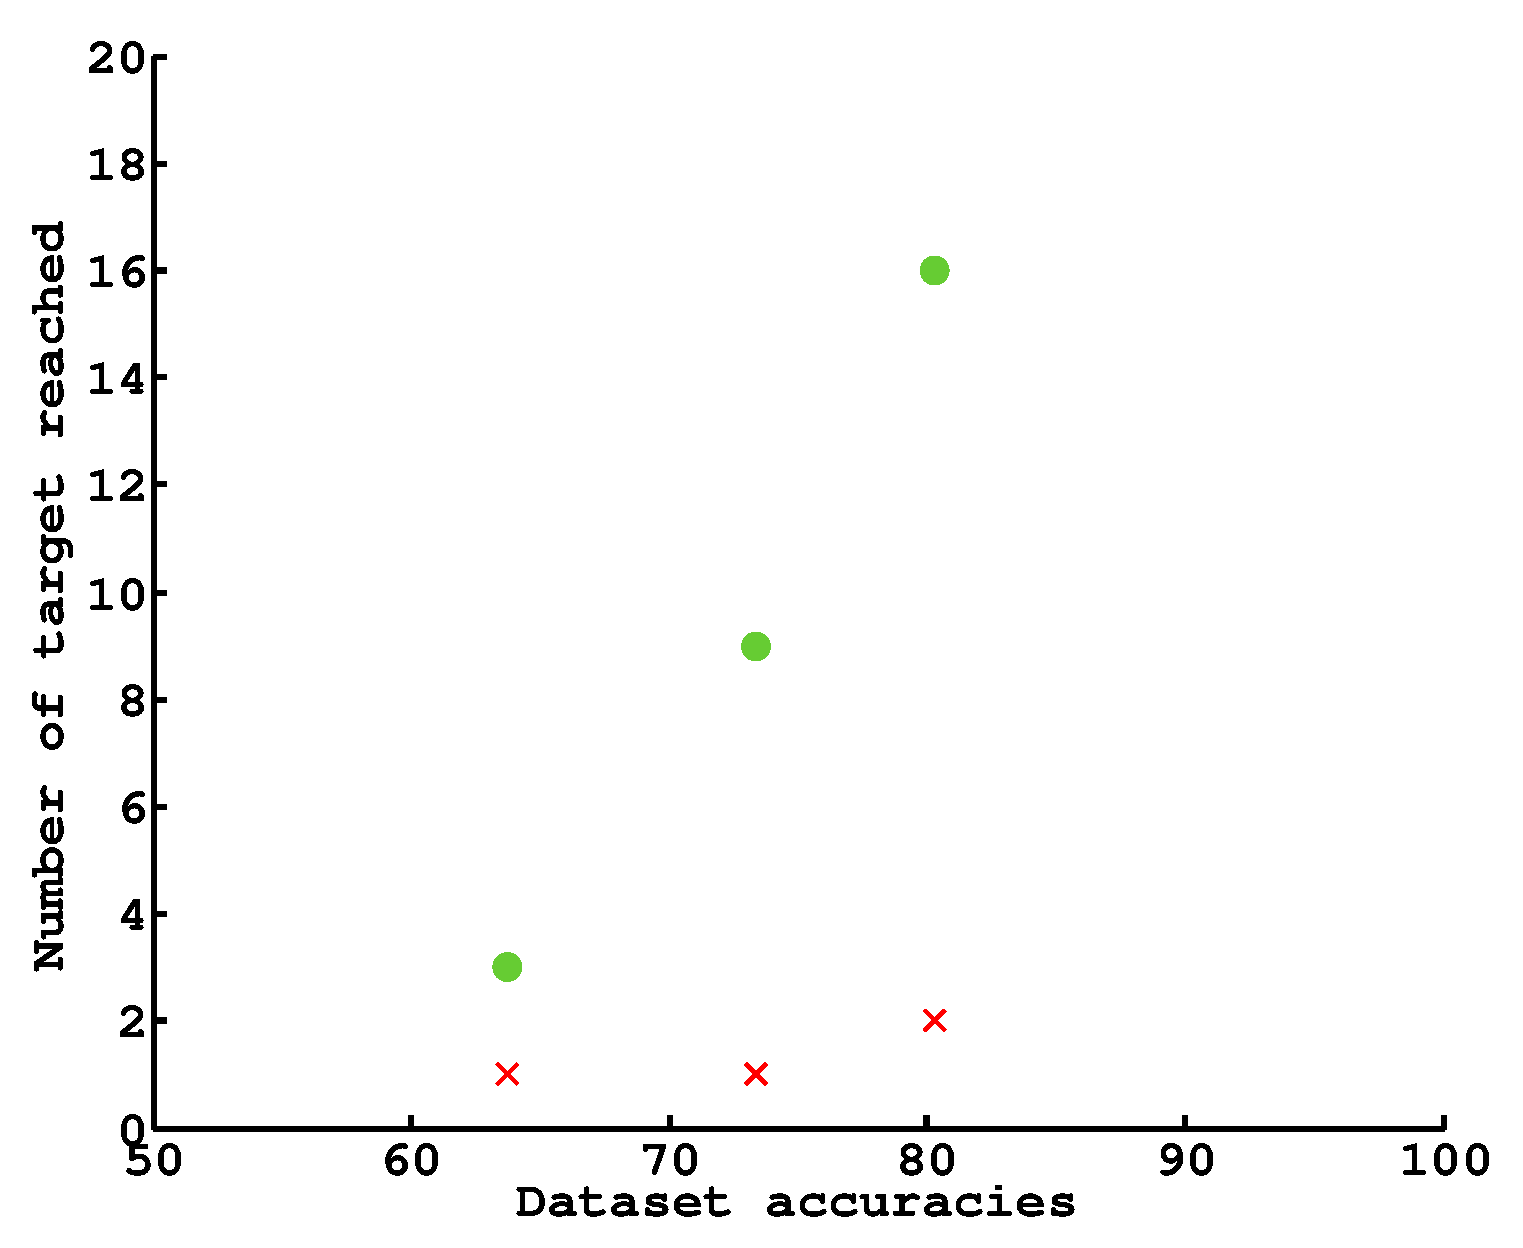
\includegraphics[width=\plotsize\columnwidth]{\imgpath/onlineXP/correct_and_error.eps}
\caption{Number of task correctly (green dot) and incorrectly (red crosses) achieved in 500+ steps during our online experiment with real subjects. We kept running the experiments after 500 steps until the systems identified the next task. Our algorithm allow a user to control online and with their brain the final position of our agent, without the need to calibrate the system beforehand. The performance of the system is also correlated with the qualities of the EEG signals and matches well with our results form our simulated experiment.}
\label{fig:correcterror_online}
\end{figure} 


\begin{figure}[!htbp]
\centering
\includegraphics[width=\plotsize\columnwidth]{\imgpath/onlineXP/timefirst.eps}
\caption{Number of steps to complete first task for all subjects in our online experiments. The results are plotted against the a posteriori computed 10 fold accuracy of our classifier on each subject EEG signals. The relation between data quality and the time to first task is in line with our simulated results shown in Figure~\ref{fig:timefirst_powermatching}. Note that this first target was always the correct one for every subject.}
\label{fig:timefirst_online}
\end{figure} 


\begin{table}
\centering
\rowcolors{2}{gray!25}{white}
\begin{tabular}{c c c c c c}
    Subject & Class. rate & Steps to first task & First correct & N. correct & N. error\\ \hline
    S1 & 80 & 101 & Yes & 16 & 2\\ 
    S2 & 73 & 131 & Yes & 9 & 1\\
    S3 & 64 & 265 & Yes & 3 & 1\\
\end{tabular}
\caption{Result from our online experiment. For each subject, we provide the classification rate our classifier would have if we knew the correct labels associated to the brain signals (Class. rate), the number of steps needed to identify the first task and if the task identified was the correct one. Finally, we give the number of task that were correctly and incorrectly identified in 500 steps.} 
\label{tab:onlineXPsummary}
\end{table}

% \begin{figure}[!htbp]
% \centering
% 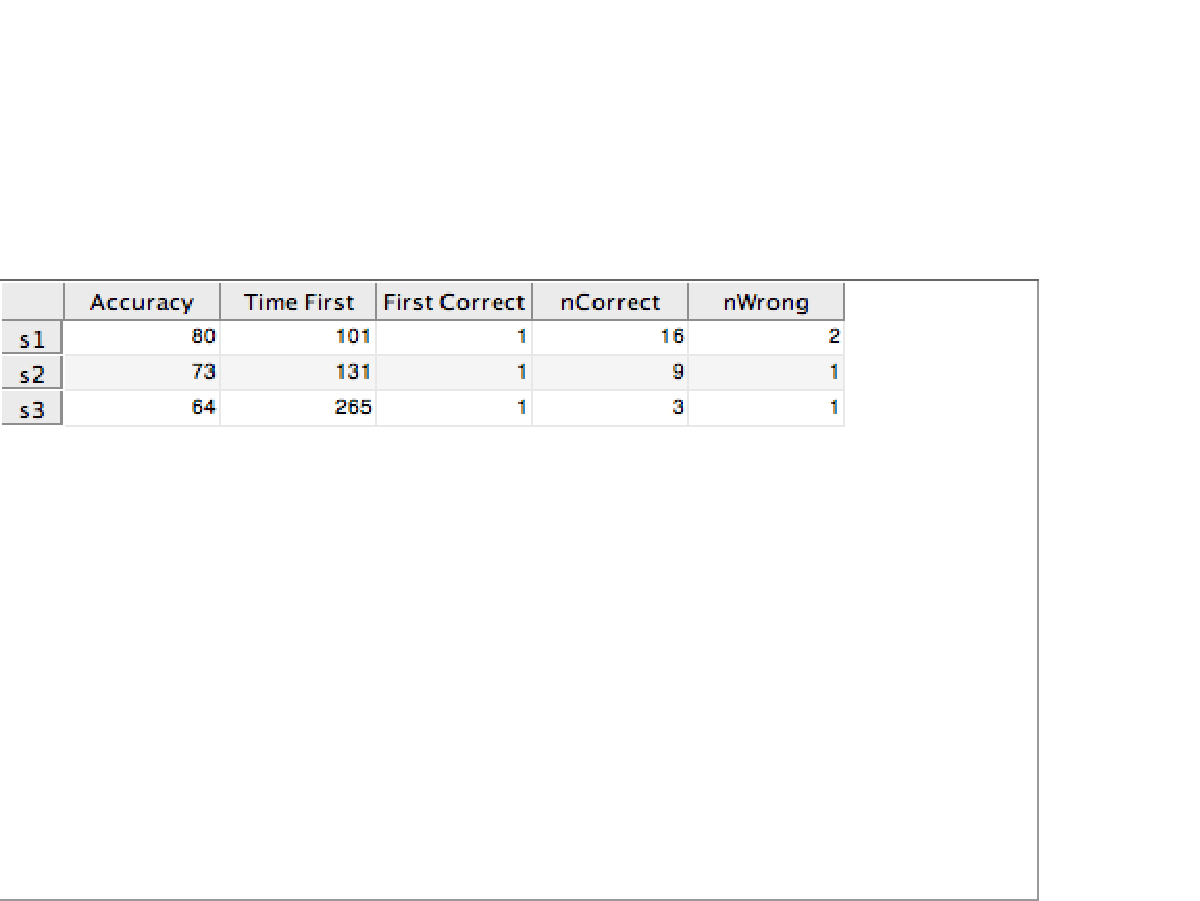
\includegraphics[width=\columnwidth]{\imgpath/onlineXP/table.png}
% \caption{\todo{change with a latex table}}
% \label{fig:correcterror_online}
% \end{figure} 

\transition

Those results with real EEG signals allow us to believe such algorithm could have practical application into the real word. By removing the user of an expert to collect and calibrate the system, we may democratize the use of brain computer interface and allow their users to go out of the labs. 

While this work offers a good solution to start interacting with systems without defining in advance the particular signals that will be used by the users, we have only demonstrated its performances on relatively simple scenario. Especially, we considered, discrete states and actions, synchronous protocol, and a finite set of task hypothesis. While those constraints are, currently, not limiting for BCI tasks, they are a more limiting factor for robotics experiments. In next chapter, we will address some of those limitations in more or less simple experiments, which may provide ideas for the future development of this work.

% accuracy = 0.83
% powerCorrect = 670
% powerWrong = 1031
% ratio = 1.54
% ratio symmetric = 0.65
% accuracy shuffle = 0.61
% ratio shuffle = 1.00


% \begin{figure}[!htbp]
% \centering
% 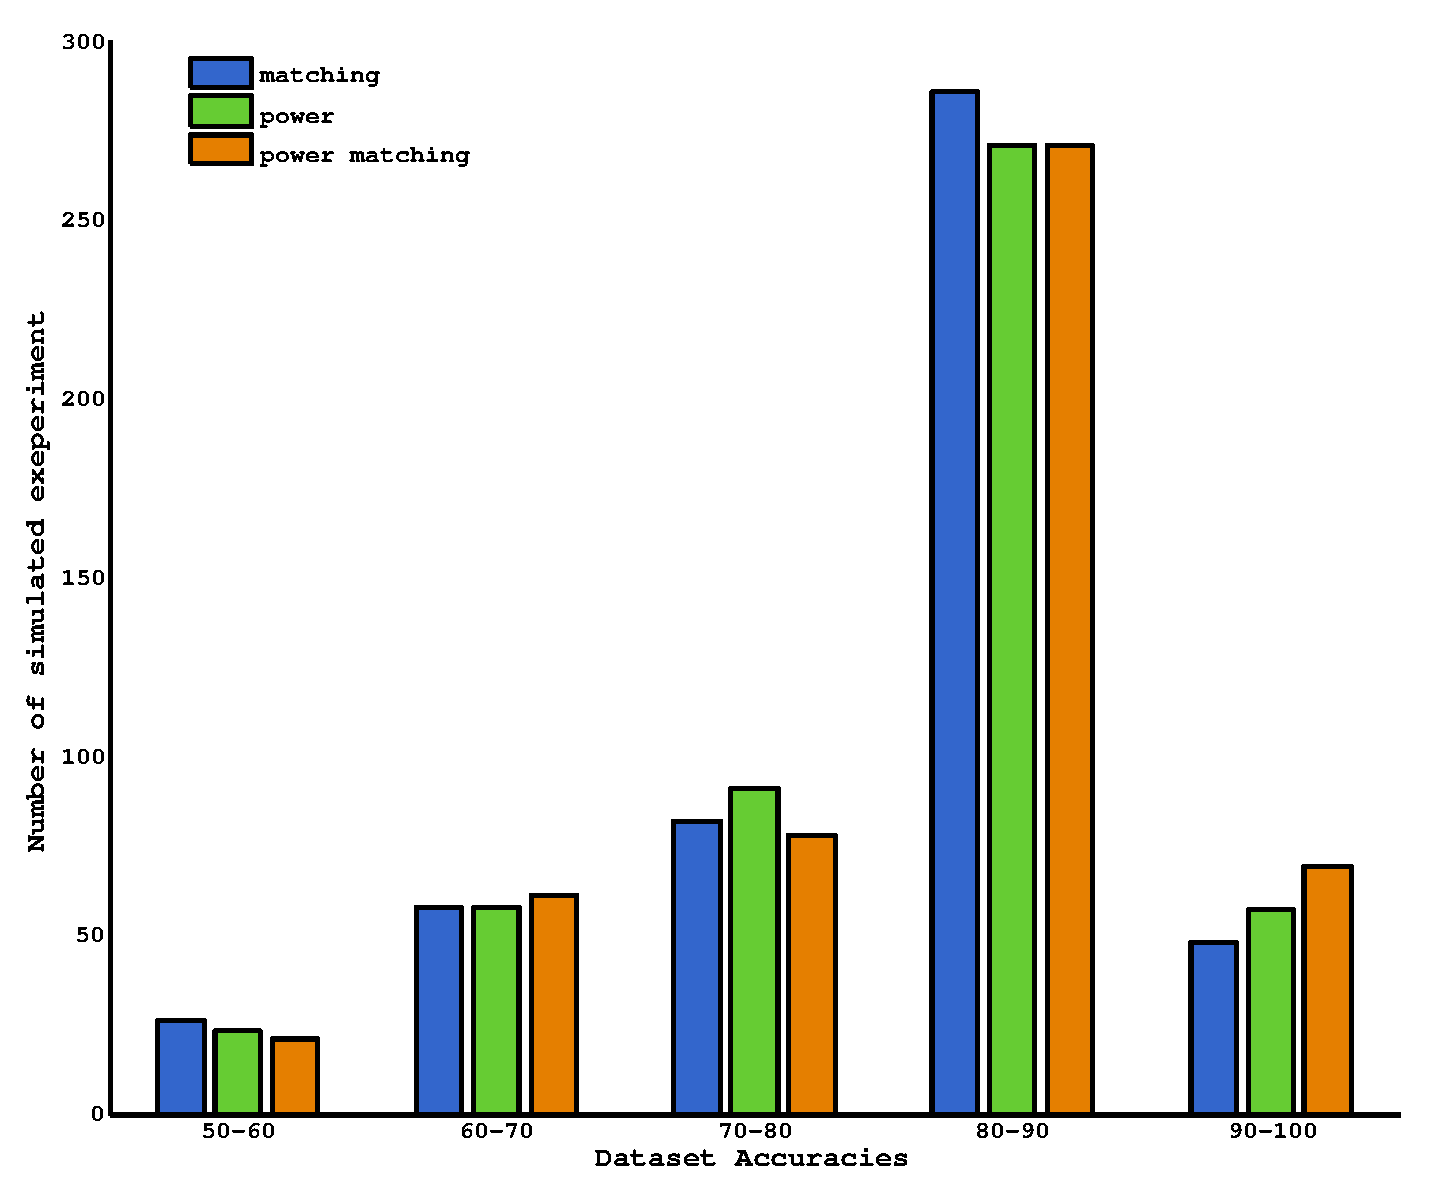
\includegraphics[width=\plotsize\columnwidth]{\imgpath/powermatching/nSim.eps}
% \caption{\todo{use a table instead of this figure}}
% \label{fig:nSim_powermatching}
% \end{figure} 


% nSim =

%   Columns 1 through 3

%     26    58    82
%     23    58    91
%     21    61    78

%   Columns 4 through 5

%    286    48
%    271    57
%    271    69

% ratioFirstWrong =

%   Columns 1 through 2

%          0         0
%     0.8261    0.1034
%     0.6190    0.0164

%   Columns 3 through 4

%          0         0
%     0.0330    0.0332
%     0.0256    0.0185

%   Column 5

%          0
%          0
%          0


% \begin{figure}[!htbp]
% \centering
% 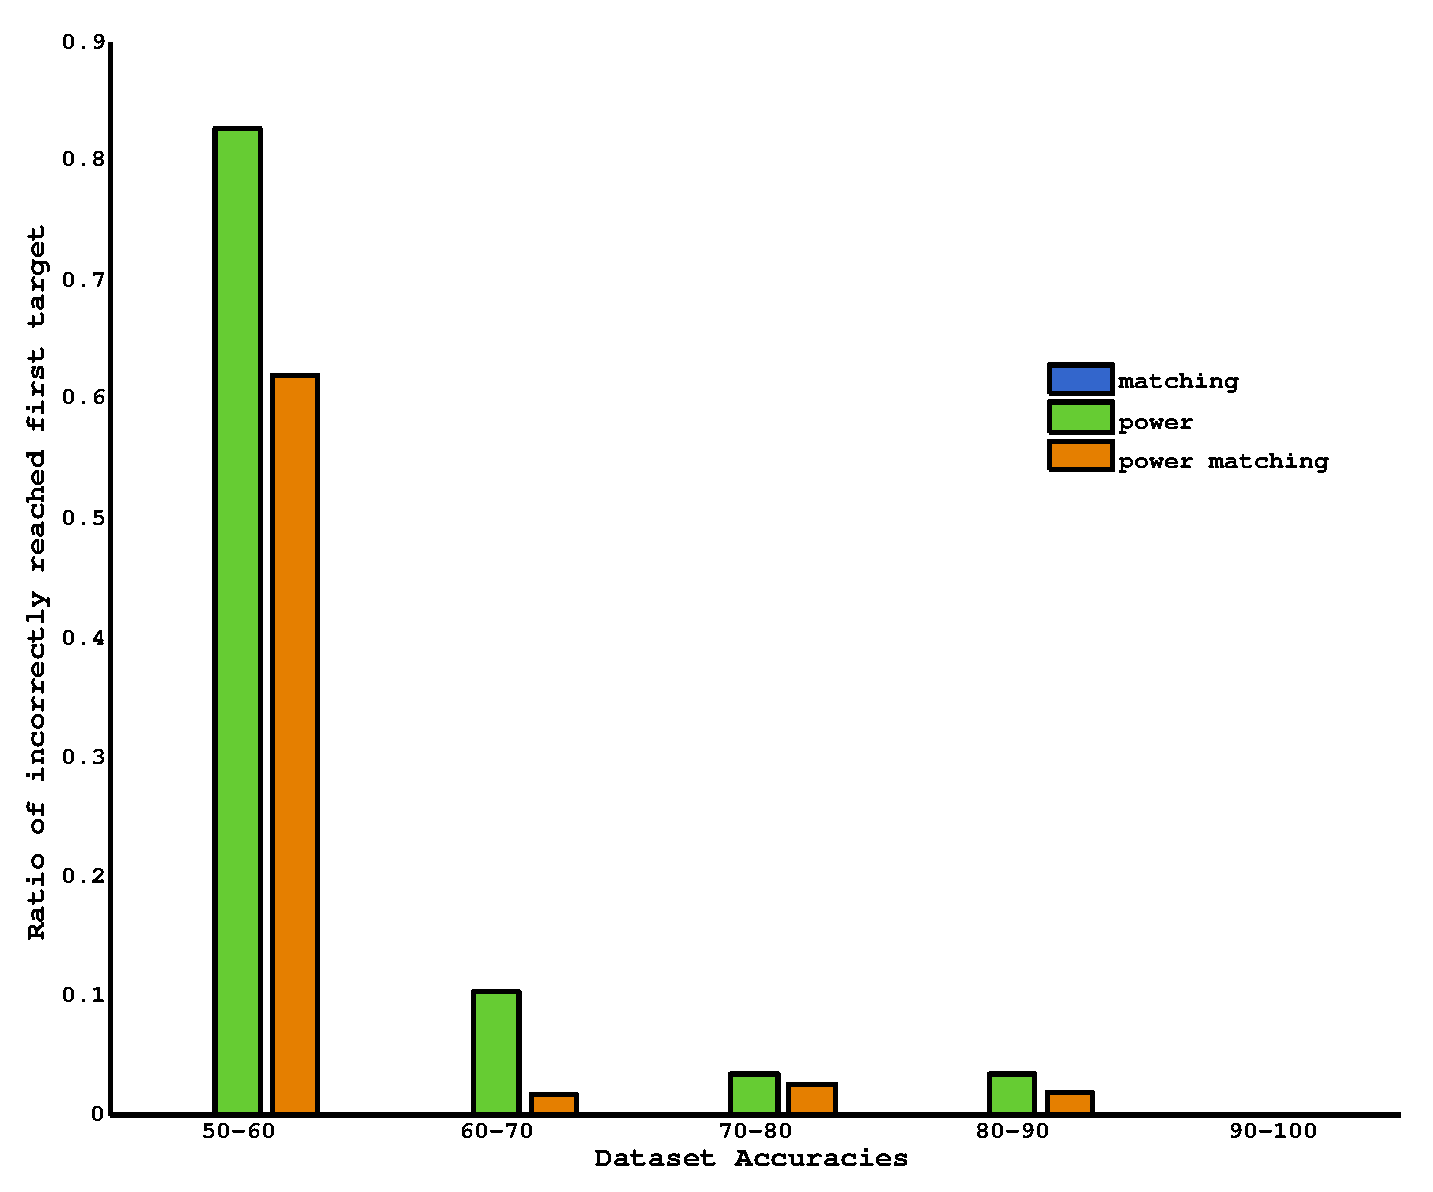
\includegraphics[width=\plotsize\columnwidth]{\imgpath/powermatching/errorfirst.eps}
% \caption{Percentage of time the first task estimated was erroneous using EEG data. Comparison between our general method (matching), or using the information that ``incorrect'' signals are more powerful than the ``correct'' (power), or both method combined (power matching). For low quality datasets, the power information increases the number of erroneous estimation. However those errors occurs for very low quality datasets, which are not the main target of our algorithm.}
% \label{fig:errorfirst_powermatching}
% \end{figure} 
